\documentclass[11pt, a4paper]{article}

% Required packages as per strict LaTeX compilation guidelines
\usepackage[a4paper, margin=2.5cm]{geometry}
\usepackage{amsmath,amssymb,booktabs,array,tabularx,enumitem}
\usepackage{tikz}
\usepackage{booktabs}
\usepackage{enumitem}
\setlist[itemize]{label=-}
\usepackage{parskip}
\usepackage{graphicx}
\usepackage{float}
\usepackage[hidelinks]{hyperref} % load last

\usetikzlibrary{arrows.meta,positioning,calc,fit,backgrounds}

\setlength{\parindent}{0pt}
\setlength{\parskip}{1em}

\begin{document}

% ---------------------------------------------------------
% TITLE PAGE
% ---------------------------------------------------------
\begin{titlepage}
    \centering
    \vspace*{2cm}
    
    {\LARGE \textbf{Lahore University of Management Sciences} \par}
    \vspace{0.5cm}
    {\Large Syed Babar Ali School of Science and Engineering \par}
    
    \vfill
    
    {\Large \textbf{AI651 --- Deep Learning for Space, Time and Graphs} \par}
    \vspace{1cm}
    {\Huge \textbf{Assignment 3 Report} \par}
    
    \vfill
    
    {\Large 
        \textbf{Student Name:} Faaiz Khan \\[0.2cm]
        \textbf{Student ID:} 25280051 
    \par}
    
    \vspace{1.5cm}
    
    % REQUIREMENT: GitHub repository link MUST be on the first page.
    {\large \textbf{GitHub Repository Link:}\\
    \vspace{0.2cm}
    \url{https://github.com/FaaizKhan1999/dl4stg-assignments} \par}
    
    \vspace*{2cm}
\end{titlepage}
% ---------------------------------------------------------

% ---------------------------------------------------------
% TASK 1
% ---------------------------------------------------------
\section*{Question 1 -- What does a sum remember?}

Throughout, a neighbourhood with $s$ slowing, $z$ steady and $p$ speeding-up sensors is described by its count triple $(s, z, p)$, with $n_v = s + z + p$ and $S_v = p - s$.

\subsection*{(a) Affine message}

With an affine message $\phi(x) = wx + c$, the aggregated message is
\[
\sum_{u \in N(v)} \phi(x_u) = \sum_{u \in N(v)} (w x_u + c) = w \sum_{u \in N(v)} x_u + c\,|N(v)| = w S_v + c\, n_v,
\]
so $h_v = \rho(w S_v + c\, n_v)$. The neighbourhood enters only through the pair $(n_v, S_v)$. If two neighbourhoods have the same $n_v$ and $S_v$, then $\rho$ receives exactly the same input, and since $\rho$ is a function it returns the same output. This holds for every choice of $w$, $c$ and $\rho$: no learnable parameter can separate them.

\textbf{Example.} $N_1 = \{-1, +1\}$ and $N_2 = \{0, 0\}$ both have $n = 2$ and $S = 0$, so both produce the aggregated message $2c$. Yet $N_1$ has no steady neighbours and $N_2$ has two. The layer cannot distinguish ``one slowing, one speeding up'' from ``both steady'', although they describe very different traffic. A numerical check with three random $(w, c)$ pairs gave identical aggregated messages for $N_1$ and $N_2$ in every case. More generally, replacing two steady sensors with one slowing and one speeding-up sensor, $(s, z, p) \to (s+1,\, z-2,\, p+1)$, leaves both $n$ and $S$ unchanged. The affine sum compresses three counts into two numbers, so the number of steady neighbours cannot in general be recovered.

\subsection*{(b) A nonlinear scalar message that remembers all three counts}

\textbf{Construction.} Let $B = K + 1$ and choose
\[
\phi(-1) = 1, \qquad \phi(0) = B, \qquad \phi(+1) = B^2 .
\]
The aggregated message is then
\[
T_v = \sum_{u \in N(v)} \phi(x_u) = s \cdot 1 + z \cdot B + p \cdot B^2 ,
\]
i.e.\ the three counts are stored in separate place values of a base-$B$ number: slowing in the units digit, steady in the $B$s digit and speeding-up in the $B^2$s digit.

\textbf{Why this is uniquely decodable.} Since $1 \le n_v \le K$, every count satisfies $0 \le s, z, p \le K = B - 1$, so each count is a valid base-$B$ digit and adding messages never produces a carry. Base-$B$ representations are unique, so different count triples always give different sums. The base cannot be smaller: if $B \le K$, then $B$ slowing neighbours $(B, 0, 0)$ and one steady neighbour $(0, 1, 0)$ are both allowed and both sum to $B$. Hence $B = K + 1$ is the smallest base that works.

\textbf{Recovering the counts.}
\[
s = T_v \bmod B, \qquad z = \left\lfloor T_v / B \right\rfloor \bmod B, \qquad p = \left\lfloor T_v / B^2 \right\rfloor .
\]

\textbf{Verification for $K = 8$.} Here $B = 9$ and $\phi(-1) = 1$, $\phi(0) = 9$, $\phi(+1) = 81$. In NumPy (\texttt{q1\_verify.py}) I enumerated all $164$ count triples with $1 \le s + z + p \le 8$, built the corresponding list of neighbour trends and summed $\phi$ over it. All $164$ sums are distinct (the largest is $8 \cdot 81 = 648$), and decoding each sum with the formulas above returns the original triple in every case.

\textbf{Counting non-steady neighbours.} Choose $\phi(x) = |x|$, i.e.\ $\phi(-1) = \phi(+1) = 1$ and $\phi(0) = 0$. Then
\[
\sum_{u \in N(v)} \phi(x_u) = s + p
\]
for any neighbourhood size, because each non-steady neighbour contributes exactly one and each steady neighbour contributes nothing. This was verified numerically for all neighbourhoods of size 1 to 29.

\subsection*{(c) Sum, mean and max with one-hot messages}

With $\phi(-1) = (1,0,0)$, $\phi(0) = (0,1,0)$, $\phi(+1) = (0,0,1)$, the three aggregators give
\[
\text{Sum} = (s, z, p), \qquad \text{Mean} = \left(\tfrac{s}{n}, \tfrac{z}{n}, \tfrac{p}{n}\right), \qquad \text{Max} = \big(\mathbb{1}[s>0],\, \mathbb{1}[z>0],\, \mathbb{1}[p>0]\big).
\]
So the sum keeps the exact counts, the mean keeps only the proportions (it loses $n$, which $\rho$ is not told), and the max keeps only which trends are present. Every entry below was also checked by brute force over all $164$ allowed neighbourhoods (\texttt{q1\_verify.py}): for each ``No'', the script found two neighbourhoods with the same aggregated vector but different correct answers.

Let $a = (a_1, a_2, a_3)$ denote the aggregated vector that $\rho$ receives.

\begin{center}
\small
\begin{tabular}{@{}lll@{}}
\toprule
Method & Possible? & Reason \\
\midrule
\multicolumn{3}{@{}l}{\textit{(i) Count steady neighbours}} \\
\addlinespace[2pt]
Sum  & \textbf{Yes} & count $= a_2$ \\
Mean & \textbf{No}  & $\{0\}$ and $\{0,0\}$ both give $(0,1,0)$; answers $1$ vs.\ $2$ \\
Max  & \textbf{No}  & $\{0\}$ and $\{0,0\}$ both give $(0,1,0)$; answers $1$ vs.\ $2$ \\
\midrule
\multicolumn{3}{@{}l}{\textit{(ii) More than half of the neighbours are slowing}} \\
\addlinespace[2pt]
Sum  & \textbf{Yes} & Yes iff $2a_1 > a_1 + a_2 + a_3$ \\
Mean & \textbf{Yes} & Yes iff $a_1 > 1/2$ \\
Max  & \textbf{No}  & $\{-1,+1\}$ and $\{-1,-1,+1\}$ both give $(1,0,1)$; answers No vs.\ Yes \\
\midrule
\multicolumn{3}{@{}l}{\textit{(iii) Any neighbour is slowing}} \\
\addlinespace[2pt]
Sum  & \textbf{Yes} & Yes iff $a_1 > 0$ \\
Mean & \textbf{Yes} & Yes iff $a_1 > 0$ \\
Max  & \textbf{Yes} & Yes iff $a_1 = 1$ \\
\bottomrule
\end{tabular}
\end{center}

\section*{Question 2 -- Which way is the slowdown moving?}

Indices are taken modulo 40 throughout. The true (backward) motion is $x_i(t+1) = x_{i+1}(t)$.

\subsection*{(a) Symmetric layer}

\textbf{(i) Fitting $a, b$ to one isolated slowdown.} Let $x_{20}(t) = 1$ and $x_j(t) = 0$ for $j \neq 20$. The layer $\hat{x}_i(t+1) = a\,x_i(t) + b\,\big(x_{i-1}(t) + x_{i+1}(t)\big)$ gives non-zero predictions only at sensors 19, 20 and 21:
\[
\hat{x}_{19} = b\,(x_{18} + x_{20}) = b, \qquad
\hat{x}_{20} = a\,x_{20} = a, \qquad
\hat{x}_{21} = b\,(x_{20} + x_{22}) = b,
\]
while the correct next snapshot is $x_{19}(t+1) = 1$ and $0$ everywhere else. All other predictions and targets are $0$, so the sum of squared errors is
\[
E(a, b) = (b - 1)^2 + a^2 + b^2 .
\]
Setting the derivatives to zero,
\[
\frac{\partial E}{\partial a} = 2a = 0 \;\Rightarrow\; a = 0, \qquad
\frac{\partial E}{\partial b} = 2(b - 1) + 2b = 0 \;\Rightarrow\; b = \tfrac{1}{2},
\]
with minimum error $E = \tfrac14 + 0 + \tfrac14 = \tfrac12$. The fitted layer predicts $0.5$ at both sensor 19 and sensor 21: because it treats both neighbours alike, it cannot tell which side the slowdown moves to, and the least-squares optimum splits the prediction evenly between them. A numerical least-squares fit (\texttt{q2\_ring.py}) gives the same values, $a = 0$, $b = 0.5$, $E = 0.5$.

\textbf{(ii) Rolling out the fitted layer.} Starting from $x_i(0) = e^{-(i-20)^2/8}$, I applied the fitted layer $\hat{x}_i(t+1) = \tfrac12\big(x_{i-1}(t) + x_{i+1}(t)\big)$ for 20 steps, feeding each prediction back as the next input, and separately applied the true shift \texttt{np.roll(x, -1)}.

\begin{figure}[H]
\centering
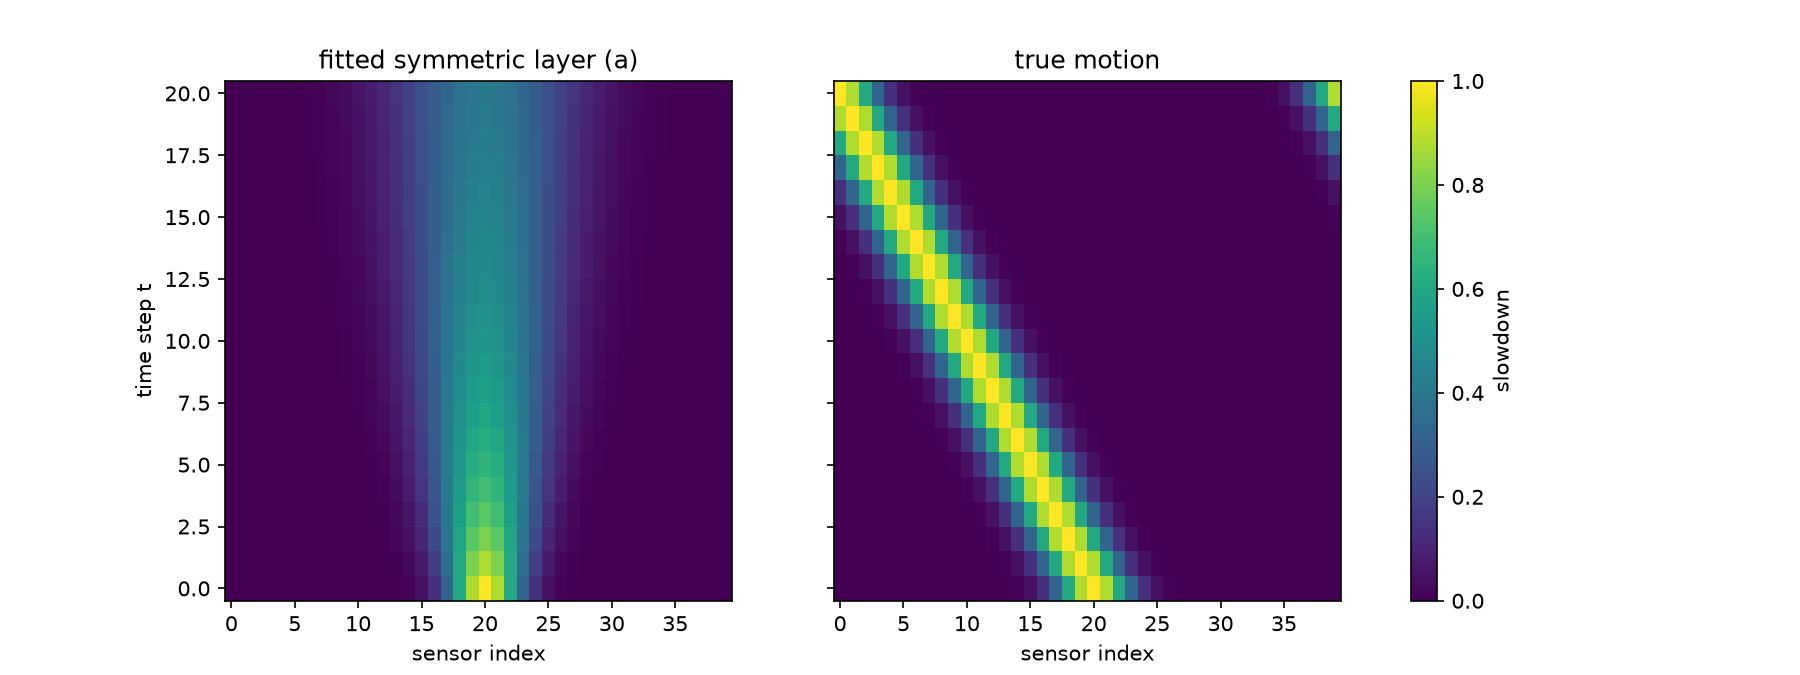
\includegraphics[width=\textwidth]{../figures/q2a_heatmaps.png}
\caption{Fitted symmetric layer (left) vs.\ true motion (right); same colour scale.}
\end{figure}

The fitted layer does not move the bump at all: its peak stays at sensor 20 while it flattens and spreads symmetrically in both directions (peak height $1.00 \to 0.53$ at $t = 10 \to 0.41$ at $t = 20$), i.e.\ it behaves like diffusion. Since $a + 2b = 1$, the total slowdown is conserved and only spread out. The true pattern instead translates one sensor per step against traffic without changing shape, keeping peak height $1$ and reaching sensor $0$ at $t = 20$.

\subsection*{(b) Direction-aware weights}

Choose $a = 0$, $w_- = 0$, $w_+ = 1$. Substituting,
\[
\hat{x}_i(t+1) = 0 \cdot x_i(t) + 0 \cdot x_{i-1}(t) + 1 \cdot x_{i+1}(t) = x_{i+1}(t) = x_i(t+1),
\]
which is exactly the true next snapshot for every input. A least-squares fit on 200 random snapshots recovers the same coefficients with error $\approx 10^{-27}$, i.e.\ zero up to floating-point precision.

The difficulty in (a) was that a layer with one shared weight $b$ for both neighbours is symmetric: mirroring the input mirrors the output, so a symmetric input (such as an isolated slowdown) must give a symmetric prediction, and the layer can never put the slowdown on one side only. With separate weights the layer is told which neighbour is ahead ($i + 1$) and which is behind ($i - 1$). This breaks the symmetry, so it can simply copy the reading from the sensor ahead.

\textbf{As a 1D convolution.} The layer is a convolution with one input and one output channel, kernel size 3 and no bias. With the kernel applied to $[x_{i-1}, x_i, x_{i+1}]$ (cross-correlation, as in PyTorch's \texttt{Conv1d}), the kernel entries are
\[
[\,w_-,\; a,\; w_+\,] = [\,0,\; 0,\; 1\,].
\]
The ring boundary is handled with circular padding of one element on each side ($x_{-1} = x_{39}$, $x_{40} = x_0$), i.e.\ \texttt{padding=1, padding\_mode="circular"} in PyTorch. With these weights, the \texttt{Conv1d} output matched the true shift up to $6 \times 10^{-8}$ (float32 rounding).

\subsection*{(c) Equal neighbour weights with history}

\textbf{(i) Backward motion.} The previous snapshot also follows $x_i(t) = x_{i+1}(t-1)$. Applying this at sensor $i - 1$ gives $x_{i-1}(t) = x_i(t-1)$: the reading that was at sensor $i$ one step ago is now at sensor $i - 1$. Hence
\[
x_i(t-1) = x_{i-1}(t).
\]
Substituting into the layer,
\[
\hat{x}_i(t+1) = a\,x_i(t) + b\,\big(x_{i-1}(t) + x_{i+1}(t)\big) + c\,x_{i-1}(t).
\]
To match the target $x_{i+1}(t)$ for every input, choose
\[
a = 0, \qquad b = 1, \qquad c = -1,
\]
which gives $\hat{x}_i(t+1) = x_{i-1}(t) + x_{i+1}(t) - x_{i-1}(t) = x_{i+1}(t) = x_i(t+1)$. A least-squares fit on random snapshot pairs recovers $a = 0$, $b = 1$, $c = -1$ with error $\approx 10^{-28}$.

\textbf{(ii) Forward motion.} Now $x_i(t+1) = x_{i-1}(t)$, and the previous snapshot satisfies $x_i(t) = x_{i-1}(t-1)$. Applying this at sensor $i + 1$ gives $x_{i+1}(t) = x_i(t-1)$, so
\[
x_i(t-1) = x_{i+1}(t).
\]
With the same coefficients,
\[
\hat{x}_i(t+1) = 0 + \big(x_{i-1}(t) + x_{i+1}(t)\big) - x_{i+1}(t) = x_{i-1}(t) = x_i(t+1).
\]
The same coefficients therefore also predict forward motion exactly (numerically, maximum error $9 \times 10^{-16}$).

\textbf{(iii) How history resolves the direction.} A single snapshot of a symmetric pattern does not say which way it is moving, which is why the symmetric layer in (a) failed. Two consecutive snapshots do: the reading that was at sensor $i$ at time $t-1$ is found at time $t$ at the neighbour \emph{towards which} the pattern moves ($i - 1$ for backward motion, $i + 1$ for forward motion). The term $c\,x_i(t-1) = -x_i(t-1)$ cancels exactly that neighbour from the symmetric sum, leaving the neighbour the pattern is \emph{coming from}, which is where sensor $i$'s next reading comes from. The spatial weights remain equal; the direction information enters through the time history, which acts like a temporal difference that reveals the velocity of the pattern. This is why spatio-temporal models combine graph aggregation with temporal encoding of several past steps.

\section*{Question 3 -- Dataset Preparation and Graph Construction}

\subsection*{Q3(a) -- Data extraction and resampling}

\textbf{Extraction.} The LargeST release provides one file per year (\texttt{ca\_\allowbreak his\_\allowbreak raw\_\allowbreak 2020.h5}, \texttt{ca\_\allowbreak his\_\allowbreak raw\_\allowbreak 2021.h5}) covering all 8{,}600 California sensors, together with the sensor metadata (\texttt{ca\_\allowbreak meta.csv}) and the road-network adjacency (\texttt{ca\_\allowbreak rn\_\allowbreak adj.npy}). The San Diego subset consists of the sensors in Caltrans District 11, which gives exactly $716$ sensors. Each yearly file stores the flow as one $T \times 8{,}600$ float64 matrix (about 7\,GB per year), which does not fit in memory. I therefore read it in blocks of 4{,}096 rows and kept only the 716 SD columns from each block (stored as float32), so peak memory stayed below 1\,GB.

\textbf{Sensor ordering.} The node order is fixed once, by the order of the SD sensors in the metadata. Flow columns are selected by matching sensor IDs against this list, and the adjacency is indexed with the same sensors' row positions. Two checks confirm the alignment: the column order of the \texttt{.h5} files equals the row order of the metadata, and the metadata field \texttt{ID2} equals each sensor's row position, which is also its row and column in the adjacency matrix.

\textbf{Time range.} The extracted data contain $210{,}528$ five-minute timestamps from 2020-01-01 00:00 to 2021-12-31 23:55. Every consecutive difference is exactly 5 minutes, so the time grid itself has no gaps (2020 is a leap year: $366 \times 288 = 105{,}408$ steps).

\textbf{Resampling to 15 minutes.} The LargeST flow values are vehicle counts per 5-minute interval, summed over lanes. The 5-minute distribution (1st/25th/50th/75th/99th percentiles: $5, 71, 182, 332, 681$) is consistent with this. Since the measurement is a count, the 15-minute value should be the \emph{sum} of the three 5-minute counts, giving units of vehicles per 15 minutes. I implemented this as
\[
X^{15\text{min}}_t = 3 \cdot \operatorname{mean}\big(\text{available values among } X^{5\text{min}}_{3t}, X^{5\text{min}}_{3t+1}, X^{5\text{min}}_{3t+2}\big),
\]
which equals the sum when all three values are present, does not underestimate the count when one or two are missing, and is missing only if all three are. The result has $70{,}176$ fifteen-minute steps (35{,}136 in 2020 and 35{,}040 in 2021) for each of the 716 sensors.

\textbf{Missing values.} At 5-minute resolution, 5.07\% of all values are missing. Table~\ref{tab:missing} shows how this is distributed across sensors.

\begin{table}[H]
\centering
\small
\begin{tabular}{@{}lr@{}}
\toprule
Sensors with no missing values & 0 \\
Sensors with $<5\%$ missing & 671 \\
Sensors with 5--50\% missing & 2 \\
Sensors with 50--$<$100\% missing & 24 \\
Sensors with no data at all (both years) & 19 \\
Sensors with no data in 2021 & 43 \\
\midrule
Exact zeros (kept as valid readings) & 0.27\% \\
\bottomrule
\end{tabular}
\caption{Missingness at 5-minute resolution.}
\label{tab:missing}
\end{table}

Three observations shaped the handling. First, no sensor is complete, which suggests network-wide outage periods that affect every sensor at once. Second, 19 sensors never report, and a further 24 stop reporting in 2021: they appear in the training year but have no test targets. Third, missingness comes in long blocks rather than isolated points. I therefore used the following procedure:
\begin{enumerate}
\item Record an observation mask of the truly observed 15-minute values before any filling.
\item Fill gaps of at most one hour (4 steps) by linear interpolation in time.
\item Set all remaining missing values to 0 and keep them marked as unobserved in the mask.
\end{enumerate}
After resampling, 94.94\% of values are observed, only 0.01\% are recovered by interpolation, and 5.05\% are zero-filled and masked. The mask is used to exclude unobserved targets from the loss and from all reported metrics, so no model is trained on or evaluated against filled values. Because the mask marks only originally observed values, the few interpolated values (0.01\%) are in the end treated like the other missing values in the forecasting pipeline: they are set to the training mean as inputs and ignored as targets. This also guarantees that no interpolated value can carry information across a split boundary. Isolated exact zeros (0.27\%) are plausible at night and were kept.

\textbf{Visualisation.} Figure~\ref{fig:week} shows the week of 3--9 February 2020 (Monday to Sunday) for three sensors: the busiest sensor with complete data (1120611), a sensor of median volume (1115972) and a sensor with gaps that week (1117931).

\begin{figure}[H]
\centering
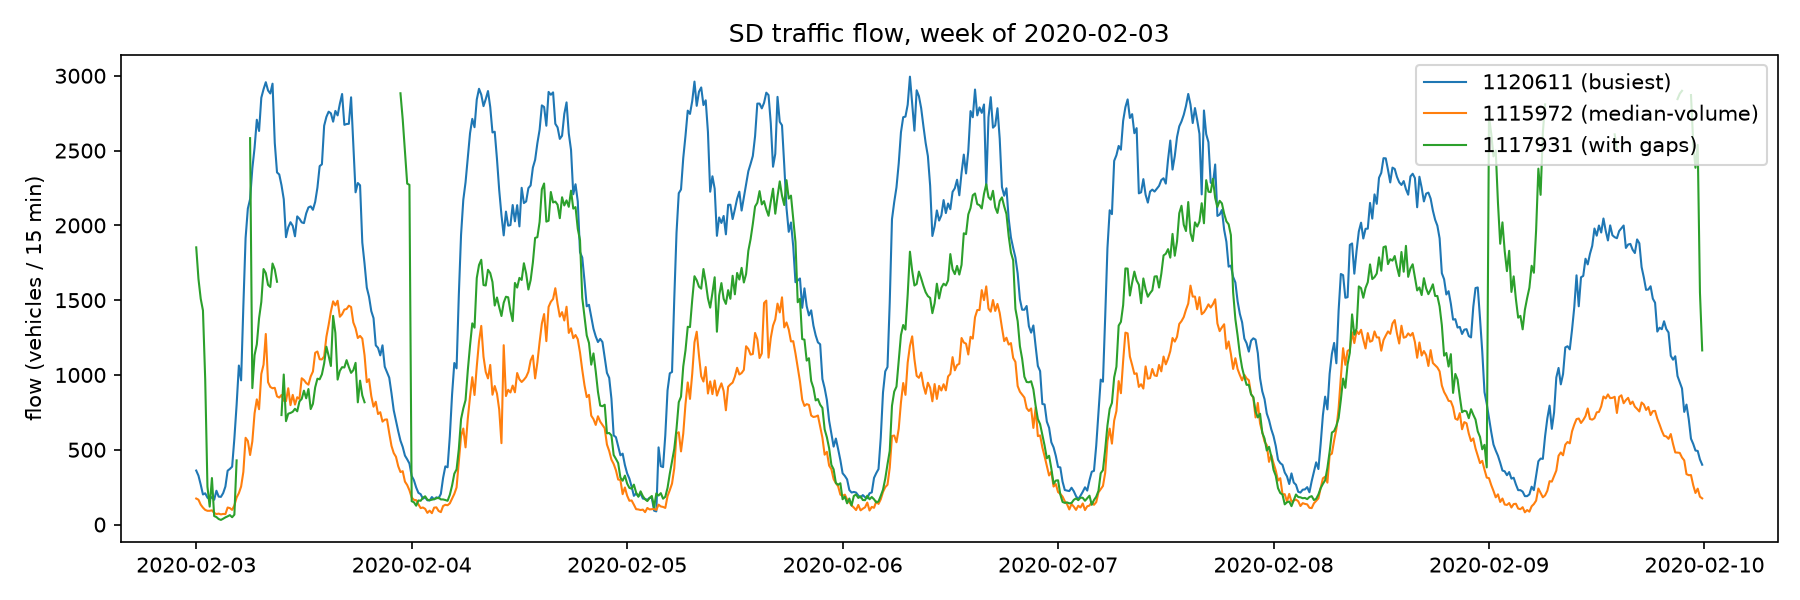
\includegraphics[width=\textwidth]{../figures/q3a_week.png}
\caption{Traffic flow of three SD sensors over one week (3--9 February 2020), 15-minute resolution.}
\label{fig:week}
\end{figure}

All sensors show a strong daily cycle, with night-time flow of roughly 100--250 vehicles per 15 minutes. On weekdays the busiest sensor has two peaks of about 2{,}900 vehicles per 15 minutes (morning and afternoon) with a dip to about 2{,}000 at midday. At the weekend the pattern changes to a single, broader and lower midday peak (about 2{,}400 on Saturday and 2{,}000 on Sunday). The median-volume sensor has a markedly stronger afternoon peak than morning peak (about 1{,}500 vs.\ 1{,}000--1{,}300), as expected for a sensor that mainly carries one direction of the commute. The third sensor shows the outages directly as breaks in the curve. Around these outages it also reports implausible values, e.g.\ more than 2{,}500 vehicles per 15 minutes around midnight on 3--4 February and in the early hours of 9 February, when the other sensors read about 200. These are faulty readings rather than missing values, so they are not caught by the mask. I did not remove outliers, and this remains a limitation of the preprocessing.

\subsection*{Q3(b) -- Constructing the traffic graph}

The adjacency submatrix $A_{SD} \in \mathbb{R}^{716 \times 716}$ was extracted from the full road-network matrix using the same sensor order as the flow tensor (see Q3(a)). Table~\ref{tab:graph} summarises its structure.

\begin{table}[H]
\centering
\small
\begin{tabular}{@{}lr@{}}
\toprule
Nodes & 716 \\
Nonzero entries (including self-loops) & 18{,}035 \\
Self-loops (diagonal, all equal to 1) & 716 \\
Directed edges (excluding self-loops) & 17{,}319 \\
Density (excluding diagonal) & 3.4\% \\
\midrule
Symmetric? & No \\
Edges whose reverse edge also exists & 13{,}608 \\
One-way edges & 3{,}711 \\
Mean $|A_{ij} - A_{ji}|$ over reciprocal pairs & 0.30 \\
\midrule
Out-degree: min / median / mean / max & 0 / 20 / 24.2 / 70 \\
In-degree: min / median / mean / max & 0 / 19 / 24.2 / 68 \\
Isolated sensors (only a self-loop) & 8 \\
\midrule
Off-diagonal weight range & 0.0100 -- 1.0 \\
\bottomrule
\end{tabular}
\caption{Structure of the San Diego road-network adjacency.}
\label{tab:graph}
\end{table}

\textbf{Symmetry.} The matrix is not symmetric, in two ways: 3{,}711 edges exist in one direction only, and even where both directions exist their weights differ by 0.30 on average. The graph is therefore treated as directed throughout, which is why a row normalisation rather than the symmetric GCN normalisation is used later (Q5(a)).

\begin{figure}[H]
\centering
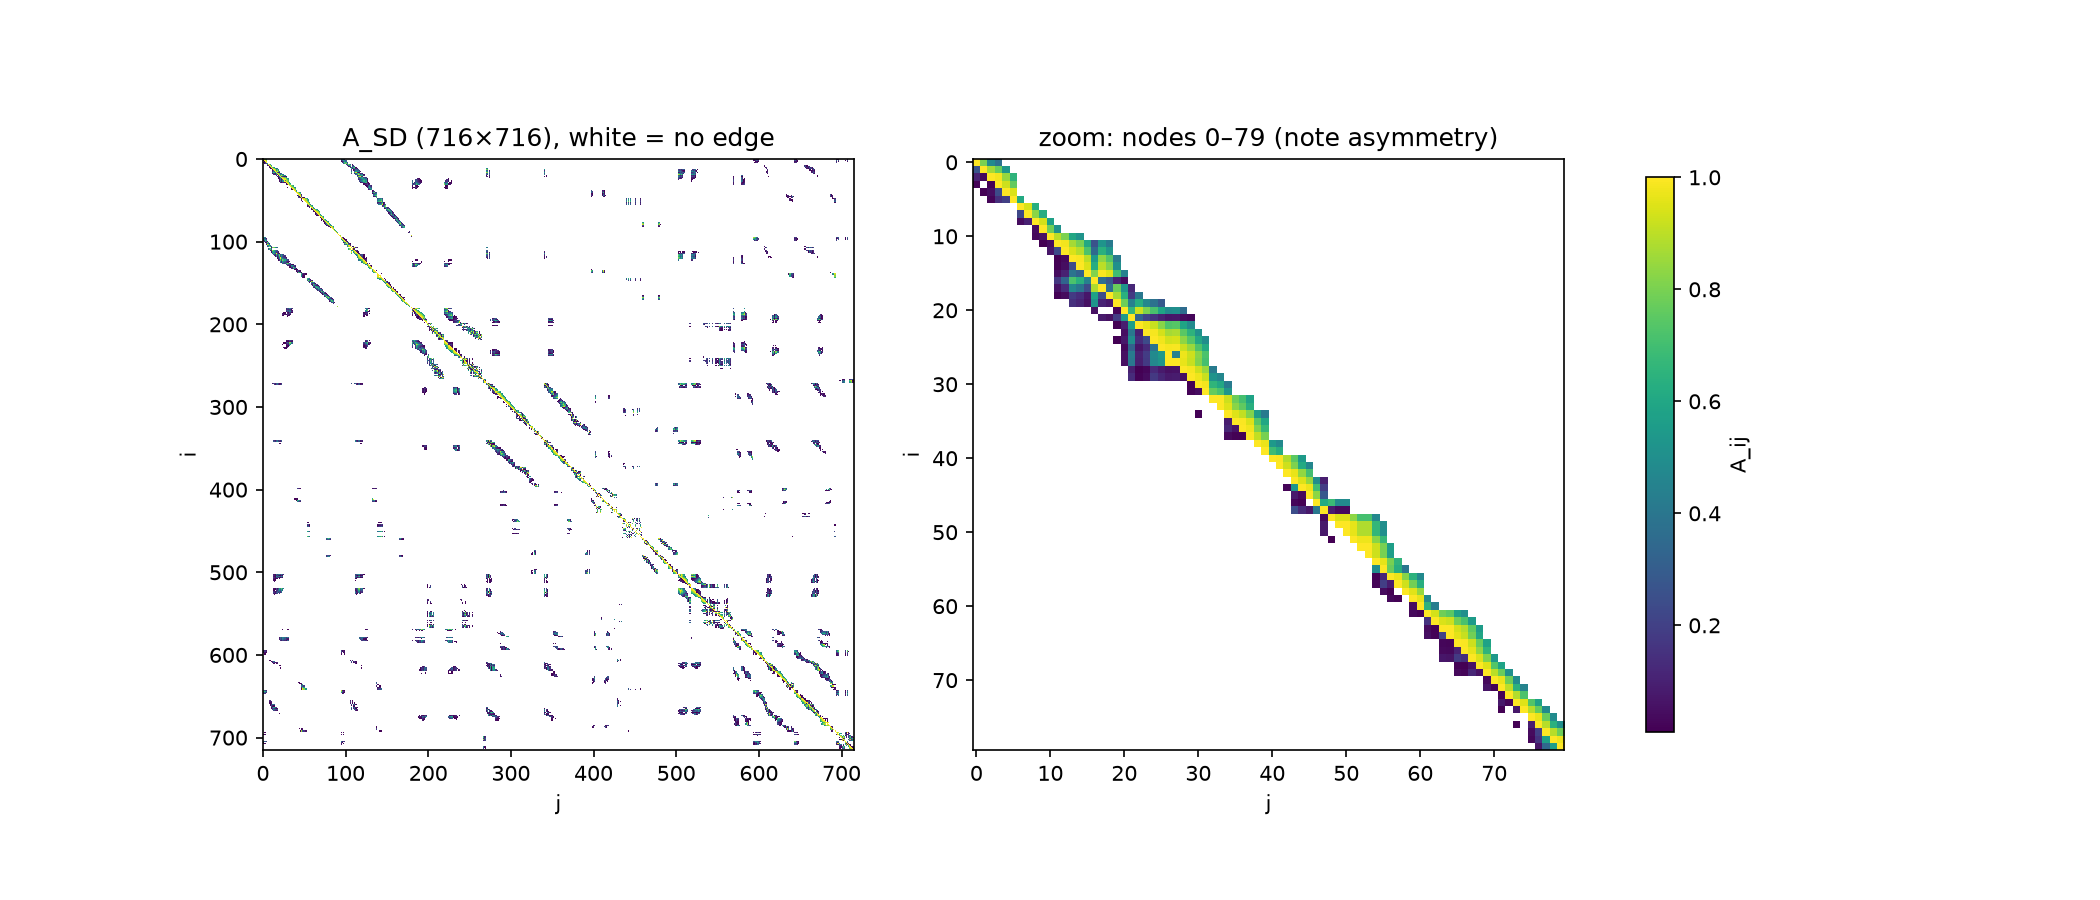
\includegraphics[width=\textwidth]{../figures/q3b_adjacency.png}
\caption{Adjacency matrix $A_{SD}$ (left; white = no edge) and a zoom on the first 80 sensors (right).}
\label{fig:adj}
\end{figure}

\textbf{Heatmap.} Figure~\ref{fig:adj} shows a strong band along the diagonal: sensors are ordered along freeways in the metadata, so consecutive sensors on the same road are connected. Bands parallel to the diagonal and scattered off-diagonal blocks connect sensors on different freeways, such as the opposite carriageway or a crossing freeway at an interchange. The zoom shows that the blocks are not mirror images of each other across the diagonal, i.e.\ the asymmetry is visible directly.

\begin{figure}[H]
\centering
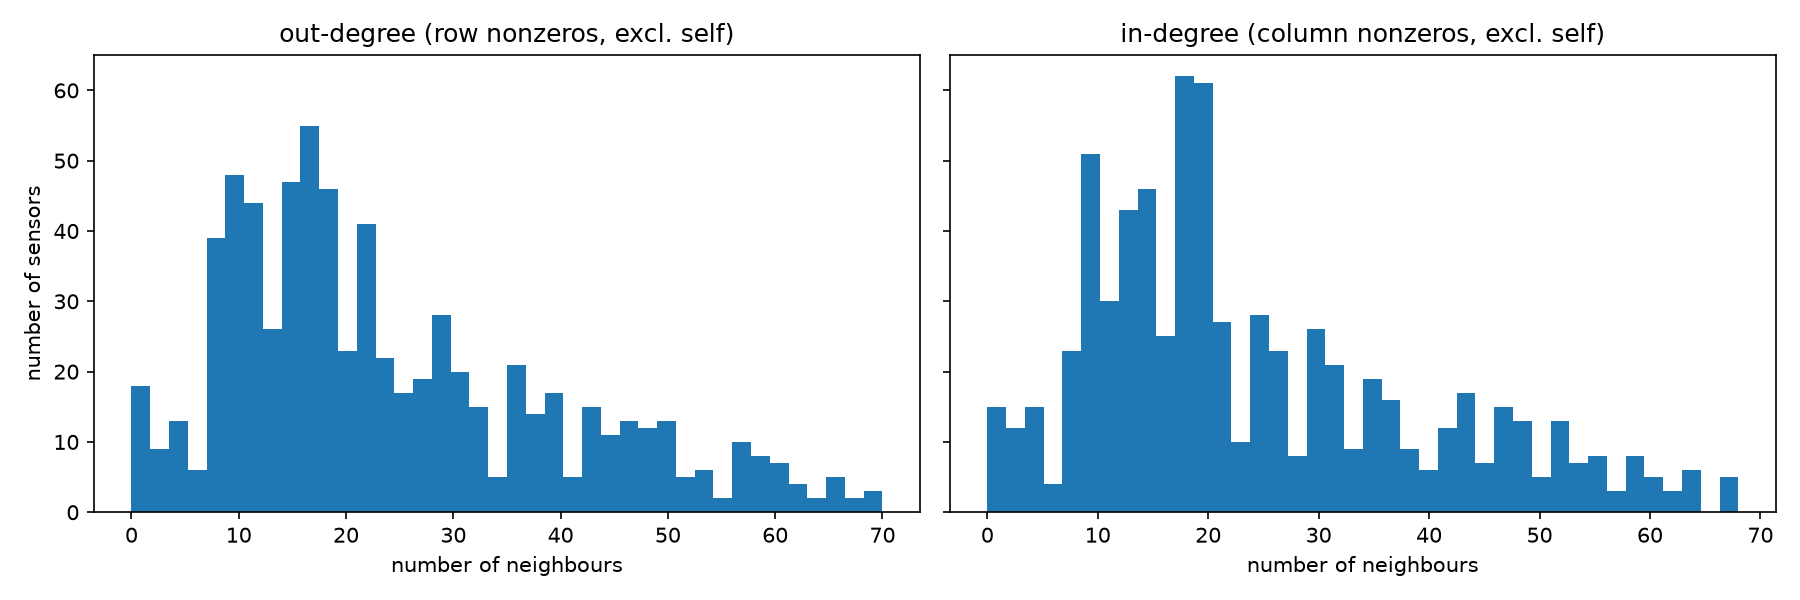
\includegraphics[width=\textwidth]{../figures/q3b_degree.png}
\caption{Distribution of out-degree (left) and in-degree (right), excluding self-loops.}
\label{fig:deg}
\end{figure}

\textbf{Degree distribution.} Both degree distributions (Figure~\ref{fig:deg}) are right-skewed: most sensors have about 8--25 neighbours, with a long tail up to 70, typically sensors near large interchanges. Eight sensors have no neighbours apart from themselves. For these, a graph convolution has nothing to aggregate, so the graph models effectively reduce to the temporal-only model at those nodes.

\textbf{Meaning of a nonzero $A_{ij}$.} The diagonal entries are all 1, and the off-diagonal weights take 5{,}207 distinct values between 0.0100 and 1. This is consistent with a Gaussian kernel of road-network distance, $A_{ij} = \exp(-d_{ij}^2 / \sigma^2)$, thresholded at about $0.01$ (as in the assignment's background section), with $d_{ii} = 0$ giving $A_{ii} = 1$. A nonzero $A_{ij}$ therefore means that sensor $j$ lies within a short driving distance of sensor $i$, and the weight is larger the shorter that distance. Because $d_{ij}$ is measured along the road network, and freeways carry traffic in one direction per carriageway, the distance from $i$ to $j$ generally differs from the distance from $j$ to $i$, which explains why $A$ is directed. I use the row of node $i$ as the set of sensors that $i$ aggregates information from.

\subsection*{Q3(c) -- Understanding graph neighbourhoods}

I selected sensor 1126411 (index 33), a 4-lane sensor on I5 northbound with less than 1\% missing data and a typical (median) out-degree. Its neighbourhoods were computed from the out-edges of the binarised adjacency (self-loop excluded): $N_1(i) = \{ j : A_{ij} \neq 0 \}$, and the two-hop neighbourhood adds every node reachable through a path of two edges.

\begin{itemize}
\item \textbf{One-hop:} 20 neighbours: 7 on I5-S, 6 on I8-E, 4 on I5-N and 3 on I8-W.
\item \textbf{Two-hop:} 53 additional sensors, i.e.\ 73 sensors within two hops.
\end{itemize}

\begin{figure}[H]
\centering
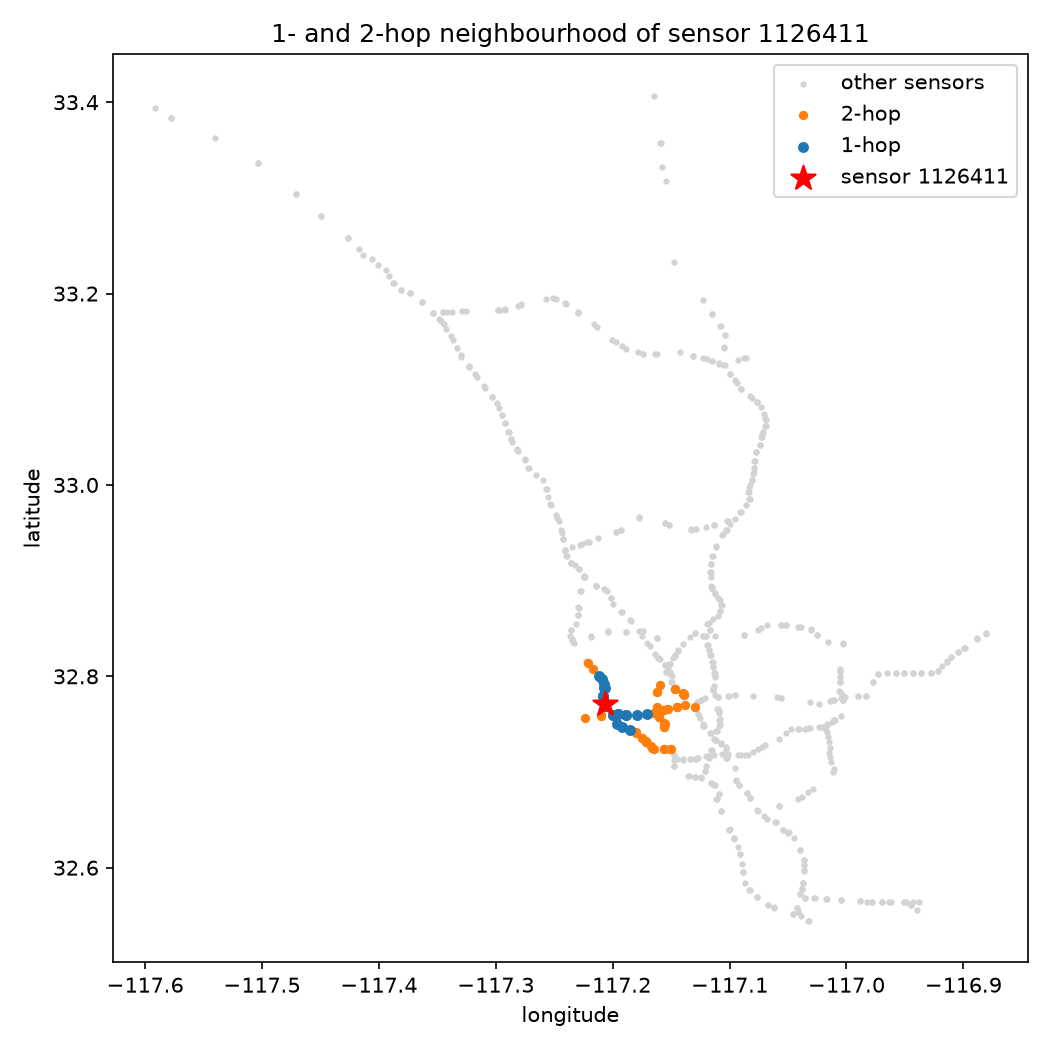
\includegraphics[width=0.6\textwidth]{../figures/q3c_neighbourhood.png}
\caption{One-hop (blue) and two-hop (orange) neighbourhood of sensor 1126411.}
\label{fig:nbhd}
\end{figure}

The sensor lies at the I5/I8 interchange (Figure~\ref{fig:nbhd}). Its one-hop neighbours are the nearby sensors along I5 in both directions and along I8 in both directions, i.e.\ the road-distance graph links not only the sensors upstream and downstream on the same carriageway, but also the opposite carriageway and the crossing freeway. The two-hop neighbourhood extends further along I5 and I8 and onto the next connecting roads.

To check whether neighbours carry information about the selected sensor, I computed the median correlation between its flow and that of its neighbours on the training year (2020, observed values only). Raw correlations are about $0.92$ for one-hop neighbours, two-hop neighbours and random non-neighbours alike, because every sensor follows the same daily cycle. After removing each sensor's average weekly profile (mean flow for each day-of-week and time-of-day), the residual correlations show the expected ordering:
\[
\text{one-hop: } 0.877 \;>\; \text{two-hop: } 0.853 \;>\; \text{random non-neighbours: } 0.800 .
\]
The random baseline remains high because 2020 contains network-wide shocks (the COVID-19 lockdown, holidays) that a year-averaged weekly profile cannot remove.

\textbf{Why might neighbouring sensors help predict traffic at the selected sensor?} Traffic is a flow along the road: a queue that forms downstream propagates back upstream, and a surge of vehicles upstream arrives at the sensor some minutes later. Neighbouring sensors therefore act as an early-warning signal for changes that the sensor's own history has not yet shown. Neighbours also share local demand (the same interchange, the same commuter flows), which is reflected in the higher residual correlation of one-hop neighbours compared with random sensors.

\textbf{What is the difference between one-hop and two-hop information aggregation?} One graph convolution layer mixes each sensor's features with those of its direct neighbours only. Stacking a second layer aggregates the already-aggregated features, so information from two hops away reaches the sensor. In general, $K$ layers give a receptive field of $K$ hops. For sensor 1126411 the neighbourhood grows from 20 sensors at one hop to 73 sensors within two hops. Two-hop aggregation adds context from further away (e.g.\ congestion approaching from several kilometres upstream), but those sensors are less strongly related, as their lower residual correlation shows.

\textbf{Could too many graph convolution layers hurt performance?} Yes:
\begin{itemize}
\item \emph{Over-smoothing.} Each layer averages features over a neighbourhood. After many layers, the features of all sensors in a connected region converge to similar values, and the model loses the sensor-specific information it needs.
\item \emph{Over-squashing.} Information from an exponentially growing number of distant sensors has to pass through a few edges, so distant signals are compressed and hard to use.
\item \emph{Harder optimisation and higher cost.} Deeper message passing is harder to train and costs more compute and memory.
\end{itemize}
The relevant dependencies for a one-hour forecast are mostly local, so one or two layers are usually enough. My own experiments show how quickly averaging can hurt: with a single graph layer but no residual connection, the sensor's own features were outweighed by its neighbours and the fixed-graph model underfit badly (test MAE 139.1 vs.\ 64.9 for temporal-only; see Q4).

% ---------------------------------------------------------
% QUESTION 4
% ---------------------------------------------------------
\section*{Question 4 -- Spatio-Temporal Traffic Forecasting}

\subsection*{Q4(a) -- Preparing forecasting windows}

Each sample uses the last 8 readings (2 hours) of all 716 sensors to predict the next 4 readings (1 hour):
\[
X_t = [x_{t-7}, \dots, x_t] \in \mathbb{R}^{8 \times 716 \times 1}, \qquad
Y_t = [x_{t+1}, \dots, x_{t+4}] \in \mathbb{R}^{4 \times 716 \times 1}.
\]

\textbf{Splits.} I first cut the 15-minute series into three time periods and only then built windows \emph{inside} each period. This way no window can contain time steps from two different splits.

\begin{table}[H]
\centering
\small
\begin{tabular}{@{}llrr@{}}
\toprule
Split & Period & Time steps & Windows \\
\midrule
Training   & 2020-01-01 -- 2020-12-31 & 35{,}136 & 35{,}125 \\
Validation & 2021-01-01 -- 2021-03-31 & 8{,}640  & 8{,}629 \\
Test       & 2021-04-01 -- 2021-12-31 & 26{,}400 & 26{,}389 \\
\bottomrule
\end{tabular}
\caption{Chronological splits. Each split loses 11 windows at its end, because a window needs 12 consecutive steps.}
\end{table}

\textbf{Normalisation.} I used a single z-score, $\tilde{x} = (x - \mu)/\sigma$, where $\mu$ and $\sigma$ are computed only from the \emph{observed} values of the training period. Validation and test data are never used to compute them. I used one global $\mu$ and $\sigma$ rather than one per sensor, because the 19 sensors without any data would have no meaningful per-sensor statistics. Missing inputs are set to $0$ after normalisation, i.e.\ to the training mean, and missing targets are ignored through the mask from Q3(a).

\subsection*{Q4(b) -- The forecasting architecture}

The model has the three required parts. All models in Q4 and Q5 use exactly this code; only the adjacency matrix changes.

\begin{enumerate}
\item \textbf{Temporal encoder.} For every sensor separately, the 8-step history goes through two 1D convolutions (kernel size 3, 32 channels, ReLU) and a linear layer that flattens the time dimension. This gives one 32-dimensional feature vector per sensor: $Z \in \mathbb{R}^{B \times 716 \times 32}$. The same encoder weights are shared by all sensors.
\item \textbf{Graph convolution.} The sensor features are mixed along the graph:
\[
H = \mathrm{ReLU}\big(\hat{A} Z W_g\big) + Z .
\]
The product $\hat{A}Z$ is taken over the sensor dimension, separately for each sample in the batch (implemented as \texttt{einsum("nm,bmd->bnd")}), so each sensor receives a weighted average of its neighbours' features. $W_g \in \mathbb{R}^{32 \times 32}$ is learned.
\item \textbf{Forecast head.} A small MLP (Linear $32 \to 32$, ReLU, Linear $32 \to 4$) maps each sensor's features $H$ to its 4 future values.
\end{enumerate}

\textbf{Why the residual ``$+\,Z$''.} The assignment's formula is $H = \mathrm{ReLU}(\hat{A} Z W_g)$. I first trained exactly this version, and the fixed-graph model failed badly: its test MAE was 139.1, more than twice the 64.9 of the temporal-only model, and its training loss stayed high, so it was underfitting rather than overfitting. The reason is that $\hat{A}Z$ \emph{replaces} each sensor's own features with an average over its row. After row normalisation, a sensor's own weight is small (median $0.14$), so its own history, which is the strongest predictor, gets drowned out by its neighbours. Some of those neighbours are on the opposite carriageway, and some are dead sensors whose input is always zero. This is over-smoothing within a single layer. Adding the residual connection keeps each sensor's own features and lets the graph add information on top. With the residual, the temporal-only model barely changed (64.9 $\to$ 64.7), while the fixed-graph model improved from 139.1 to 59.7. I kept the residual for all models, so the comparison stays fair.

\textbf{Training setup.}
\begin{itemize}
\item Loss: mean absolute error on normalised values, computed only over observed targets (masked MAE).
\item Optimiser: Adam with learning rate $10^{-3}$, batch size 64 (549 batches per epoch), gradient clipping at norm 5.
\item Epochs: 30, with early stopping on validation MAE (patience 5). The checkpoint with the best validation MAE is used for testing.
\item Hidden size $d = 32$; the temporal-only and fixed-graph models have 13{,}668 parameters.
\item Metrics: predictions are converted back to vehicles per 15 minutes before computing MAE and RMSE, again only over observed targets.
\end{itemize}

\textbf{Results of the fixed-graph STGNN.} Validation MAE $51.03$, RMSE $82.32$; test MAE $59.67$, RMSE $93.93$ (vehicles per 15 minutes). For scale, a typical 15-minute flow is around 550 vehicles, so the average error is roughly 10\%. All models do worse on the test period than on validation. The test period (April--December 2021) covers different seasons than validation (January--March), and traffic was still recovering from the 2020 lockdown, so it differs more from the training year.

\subsection*{Q4(c) -- Temporal-only baseline}

The temporal-only model uses the same encoder, the same $W_g$ and the same head, but skips the graph step: $H = \mathrm{ReLU}(Z W_g) + Z$. It therefore has exactly the same number of parameters as the fixed-graph model, and any difference comes from the graph alone.

\begin{table}[H]
\centering
\small
\begin{tabular}{@{}lrrrrrr@{}}
\toprule
& \multicolumn{2}{c}{Test overall} & \multicolumn{4}{c}{Test MAE by horizon} \\
\cmidrule(lr){2-3}\cmidrule(l){4-7}
Model & MAE & RMSE & 15 min & 30 min & 45 min & 60 min \\
\midrule
Temporal-only     & 64.66 & 101.44 & 44.90 & 58.34 & 71.44 & 83.98 \\
STGNN, fixed graph & 59.67 & 93.93  & 42.54 & 54.42 & 65.47 & 76.25 \\
\midrule
Improvement        & 7.7\% & 7.4\% & 5.3\% & 6.7\% & 8.4\% & 9.2\% \\
\bottomrule
\end{tabular}
\caption{Temporal-only vs.\ fixed-graph model on the test set.}
\end{table}

\textbf{Does modelling space help?} Yes. Using the road graph lowers the test MAE by 7.7\% and the RMSE by 7.4\%, with the same number of parameters. The gain grows with the forecast horizon: 5\% at 15 minutes but 9\% at 60 minutes. For a 15-minute forecast, a sensor's own recent history already says most of what is needed. For a 1-hour forecast, what is happening at nearby sensors now (for example a queue building up downstream) carries information that the sensor itself has not seen yet. There is one important condition: the graph only helped once each sensor's own features were kept through the residual connection. Without it, aggregating over the graph made the model much worse than ignoring the graph entirely.

% ---------------------------------------------------------
% QUESTION 5
% ---------------------------------------------------------
\section*{Question 5 -- Fixed versus Learnable Adjacency Matrices}

All experiments in this question use the same encoder, head, splits, loss, optimiser, 30-epoch budget and random seed as Q4. Only the matrix $\hat{A}$ in the graph layer changes. All models were trained on the same GPU (one NVIDIA Tesla T4), so the training times can be compared directly.

\subsection*{Q5(a) -- Fixed adjacency}

The road-network matrix is directed (Q3(b)), so the symmetric formula $D^{-1/2}(A + I)D^{-1/2}$ does not apply. I used \textbf{row normalisation} instead:
\[
\hat{A}_{\text{fixed}} = D^{-1} A, \qquad D_{ii} = \sum_j A_{ij}.
\]
Each row then sums to 1, so every sensor computes a weighted \emph{average} of the sensors in its row. I did \emph{not} add $I$: the diagonal of $A$ is already 1, and adding $I$ would double every sensor's self-weight. Every row has at least its self-loop, so $D_{ii} \geq 1$ and the division is always defined, including for the 8 isolated sensors. The matrix is stored as a fixed buffer and never changes during training.

\textbf{Result:} test MAE $59.67$, RMSE $93.93$; training time $10.4$ minutes (about 21 seconds per epoch).

\subsection*{Q5(b) -- Learnable (adaptive) adjacency}

\textbf{Implementation.} I created two trainable embedding matrices $E_1, E_2 \in \mathbb{R}^{716 \times 10}$ ($d_e = 10$), initialised from a standard normal distribution. In every forward pass the adjacency is rebuilt from them:
\[
\hat{A}_{\text{adaptive}} = \mathrm{Softmax}_{\text{row}}\big(\mathrm{ReLU}(E_1 E_2^{\top})\big).
\]
$E_1 E_2^\top$ gives a score for every pair of sensors, ReLU removes negative scores, and the row-wise softmax turns each row into weights that sum to 1, just like the row-normalised fixed graph. Because the matrix is built from $E_1$ and $E_2$ inside the forward pass, the loss gradient flows back into both embeddings, and the graph is learned together with the rest of the model. Nothing forces the learned graph to follow the roads, so it can connect any two sensors. The embeddings add $2 \times 716 \times 10 = 14{,}320$ parameters, so this model has 27{,}988 parameters in total, about twice as many as the fixed-graph model.

\textbf{Sparsification.} I used the full (dense) matrix, without keeping only the top-$k$ neighbours. A $716 \times 716$ matrix has only about half a million entries, which is cheap on a GPU, so sparsification was not needed for speed. My code supports it as an option: the scores outside each row's top $k$ are set to $-\infty$ \emph{before} the softmax, so they become exactly 0, and the remaining $k$ weights are re-normalised to sum to 1. Gradients then flow only through the kept entries. The choice of which $k$ entries to keep is not differentiable, but it is recomputed in every forward pass, so the set of kept neighbours can change as the embeddings are trained.

\textbf{Result:} test MAE $51.77$, RMSE $82.41$; training time $10.9$ minutes (about 22 seconds per epoch).

\begin{figure}[H]
\centering
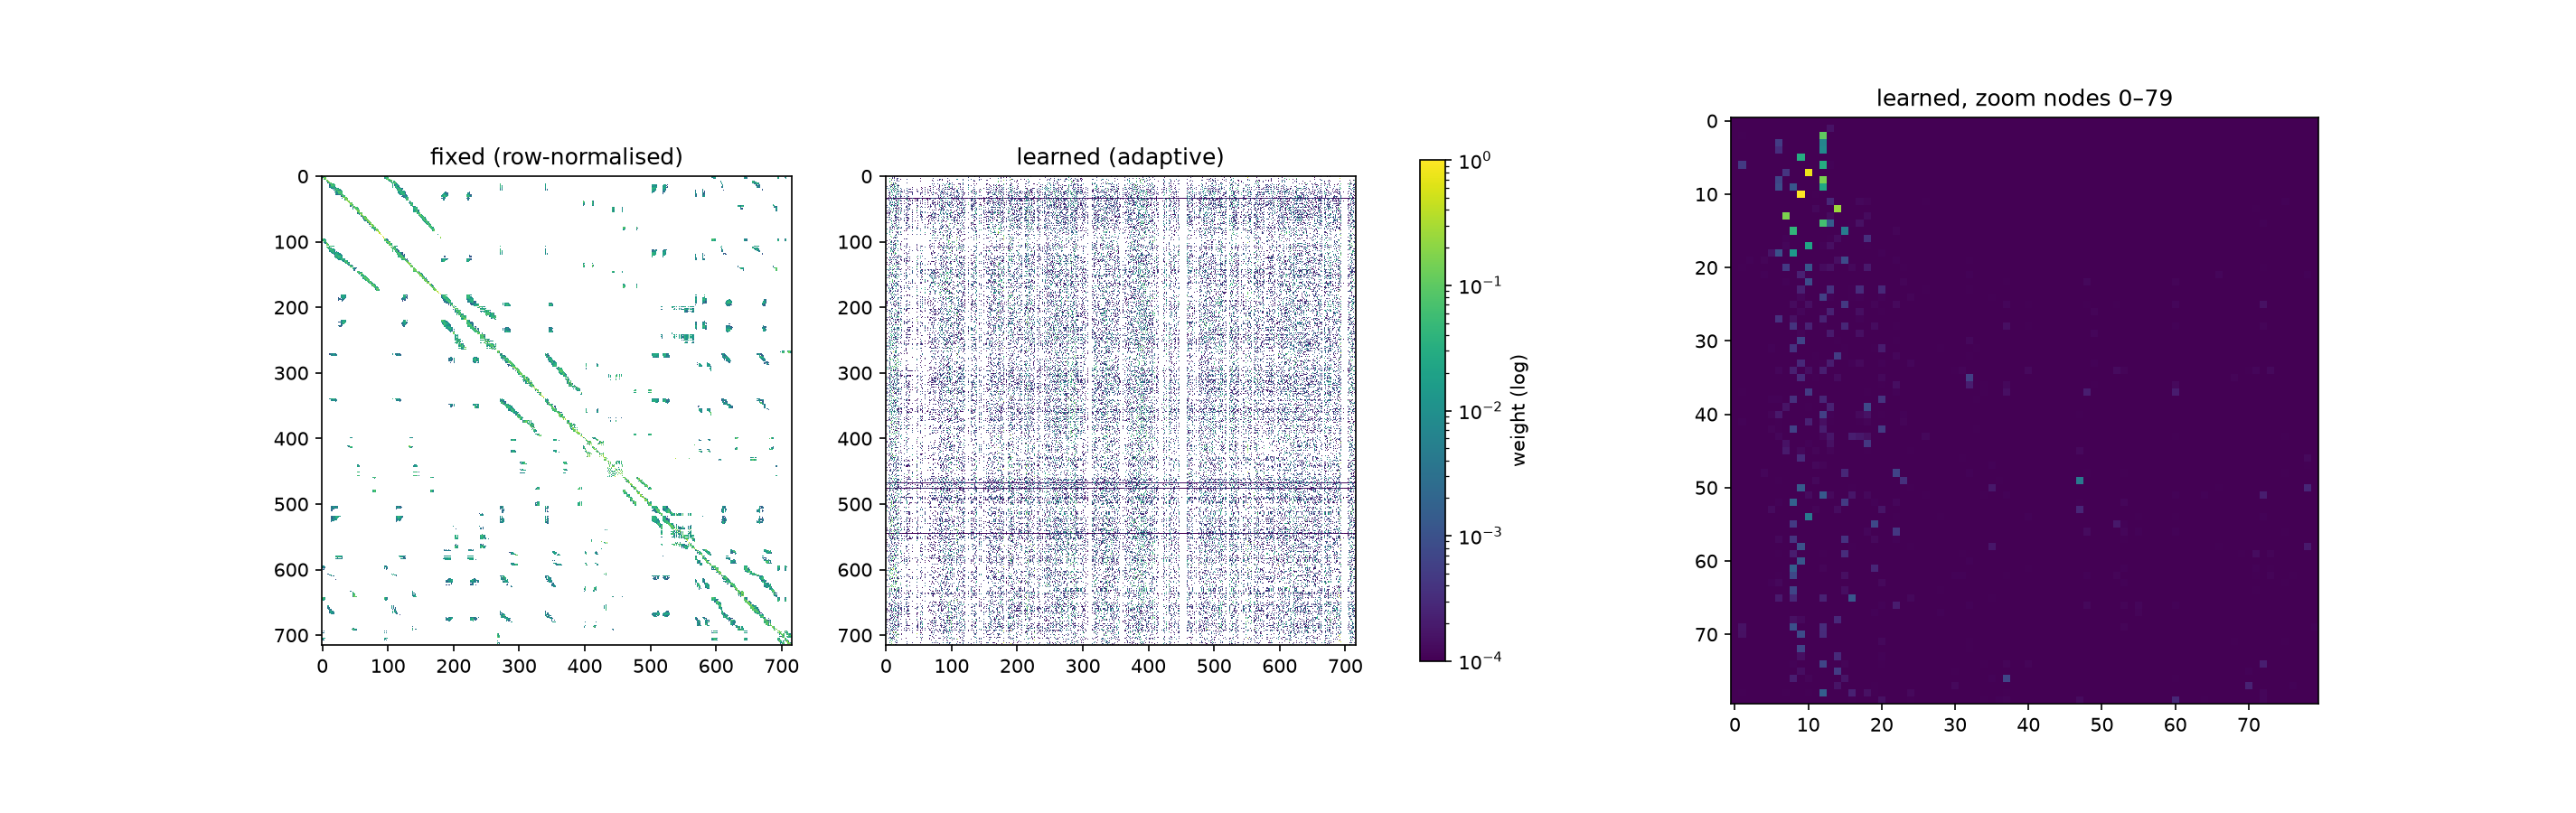
\includegraphics[width=\textwidth]{../figures/q5b_adjacency_fixed_vs_learned.png}
\caption{Fixed row-normalised adjacency (left) vs.\ learned adjacency (middle), both on a log colour scale (white: weight below $10^{-4}$), and a zoom on the learned matrix for sensors 0--79 (right).}
\label{fig:learnedadj}
\end{figure}

\textbf{What the learned graph looks like.} Figure~\ref{fig:learnedadj} shows that the two matrices look completely different. The fixed graph is sparse and follows the diagonal bands of the road network. The learned graph has no diagonal structure at all. Instead it shows \emph{vertical stripes}: certain columns receive weight from almost every row. In other words, a small number of ``hub'' sensors are used by many other sensors. The zoom makes this clearer: most of the weight in rows 0--79 goes to a handful of columns. Q6(b) analyses this in detail.

\textbf{Comparison with the fixed graph.} The learned graph is clearly better: the test MAE drops from 59.67 to 51.77 (13\% lower) and the RMSE from 93.93 to 82.41. It also improves on the temporal-only model by 20\%. Part of this gain may come from the extra 14{,}320 parameters, which the fixed-graph model does not have.

\subsection*{Q5(c) -- Hybrid adjacency}

\textbf{Implementation.}
\[
\hat{A}_{\text{hybrid}} = \alpha\, \hat{A}_{\text{fixed}} + (1 - \alpha)\, \hat{A}_{\text{adaptive}} .
\]
Both parts are normalised the same way (every row sums to 1), so the mixture also has rows summing to 1 for any $\alpha \in [0,1]$. I ran it in two ways:
\begin{itemize}
\item \textbf{Learned $\alpha$:} $\alpha = \mathrm{sigmoid}(\theta)$ with a trainable $\theta$, starting at $\alpha = 0.5$. The sigmoid keeps $\alpha$ between 0 and 1.
\item \textbf{Fixed $\alpha = 0.5$:} an equal mix of the road graph and the learned graph.
\end{itemize}

\textbf{What happened to $\alpha$.} When the model was allowed to choose, $\alpha$ fell from $0.5$ to $0.015$. The model put 98.5\% of the weight on the learned graph and almost switched the road graph off.

\begin{table}[H]
\centering
\small
\begin{tabular}{@{}lrrrrr@{}}
\toprule
Adjacency & Test MAE & Test RMSE & Val MAE & Params & Training time \\
\midrule
Fixed                     & 59.67 & 93.93 & 51.03 & 13{,}668 & 10.4 min \\
Adaptive                  & \textbf{51.77} & \textbf{82.41} & 43.58 & 27{,}988 & 10.9 min \\
Hybrid, learned $\alpha$ ($\to 0.015$) & 52.40 & 83.47 & \textbf{43.49} & 27{,}989 & 10.9 min \\
Hybrid, $\alpha = 0.5$    & 53.92 & 85.65 & 45.98 & 27{,}988 & 10.7 min \\
\bottomrule
\end{tabular}
\caption{Fixed, adaptive and hybrid adjacency (same architecture, training budget and seed).}
\end{table}

\textbf{Comparison.}
\begin{itemize}
\item Every graph that includes learned connections beats the fixed road graph by a wide margin (MAE 52--54 vs.\ 59.7).
\item The hybrid with learned $\alpha$ is practically the same model as the adaptive one, since $\alpha$ ended near 0. It is slightly better on validation (43.49 vs.\ 43.58) and slightly worse on test (52.40 vs.\ 51.77). This difference is small and probably within run-to-run noise.
\item Forcing an equal mix ($\alpha = 0.5$) is worse than both: test MAE 53.92. Giving the road graph more weight hurt, which agrees with the learned $\alpha$ choosing to ignore it.
\item Training times are almost the same for all models (10.4--10.9 minutes). Most of the computation is in the temporal encoder, which processes 716 sensor histories per sample. Building and applying a $716 \times 716$ matrix adds very little on a GPU.
\end{itemize}

In this setup, therefore, the learned graph does all the useful work, and the physical road graph adds nothing on top of it. Q6 looks at why.

% ---------------------------------------------------------
% QUESTION 6
% ---------------------------------------------------------
\section*{Question 6 -- Experimental Analysis and Interpretation}

\subsection*{Q6(a) -- Forecasting comparison}

\begin{table}[H]
\centering
\small
\begin{tabular}{@{}llrrr@{}}
\toprule
Model & Adjacency & MAE & RMSE & Training time \\
\midrule
Temporal-only & None & 64.66 & 101.44 & 10.0 min \\
STGNN & Fixed & 59.67 & 93.93 & 10.4 min \\
STGNN & Adaptive & \textbf{51.77} & \textbf{82.41} & 10.9 min \\
STGNN & Hybrid (learned $\alpha = 0.015$) & 52.40 & 83.47 & 10.9 min \\
STGNN & Hybrid ($\alpha = 0.5$) & 53.92 & 85.65 & 10.7 min \\
\bottomrule
\end{tabular}
\caption{Test results (April--December 2021), in vehicles per 15 minutes, averaged over all four horizons and all observed targets. All models trained for 30 epochs on one NVIDIA Tesla T4.}
\label{tab:final}
\end{table}

\begin{table}[H]
\centering
\small
\begin{tabular}{@{}lrrrr@{}}
\toprule
Adjacency & 15 min & 30 min & 45 min & 60 min \\
\midrule
None                        & 44.90 & 58.34 & 71.44 & 83.98 \\
Fixed                       & 42.54 & 54.42 & 65.47 & 76.25 \\
Adaptive                    & \textbf{39.66} & \textbf{48.56} & \textbf{55.91} & \textbf{62.95} \\
Hybrid (learned $\alpha$)   & 39.81 & 49.17 & 56.72 & 63.88 \\
Hybrid ($\alpha = 0.5$)     & 40.78 & 50.12 & 58.32 & 66.47 \\
\bottomrule
\end{tabular}
\caption{Test MAE for each forecast horizon.}
\label{tab:horizon}
\end{table}

\textbf{Main observations.}
\begin{itemize}
\item The ranking is the same at every horizon: adaptive is best, followed by the two hybrids, then the fixed graph, and the temporal-only model is worst.
\item The benefit of graph information grows with the horizon. At 15 minutes the adaptive model is 12\% better than temporal-only; at 60 minutes it is 25\% better. The temporal-only error almost doubles from 15 to 60 minutes (44.9 $\to$ 84.0), while the adaptive error grows much more slowly (39.7 $\to$ 63.0).
\item The extra cost is small: the best model trains less than a minute slower than the temporal-only one.
\end{itemize}

\begin{figure}[H]
\centering
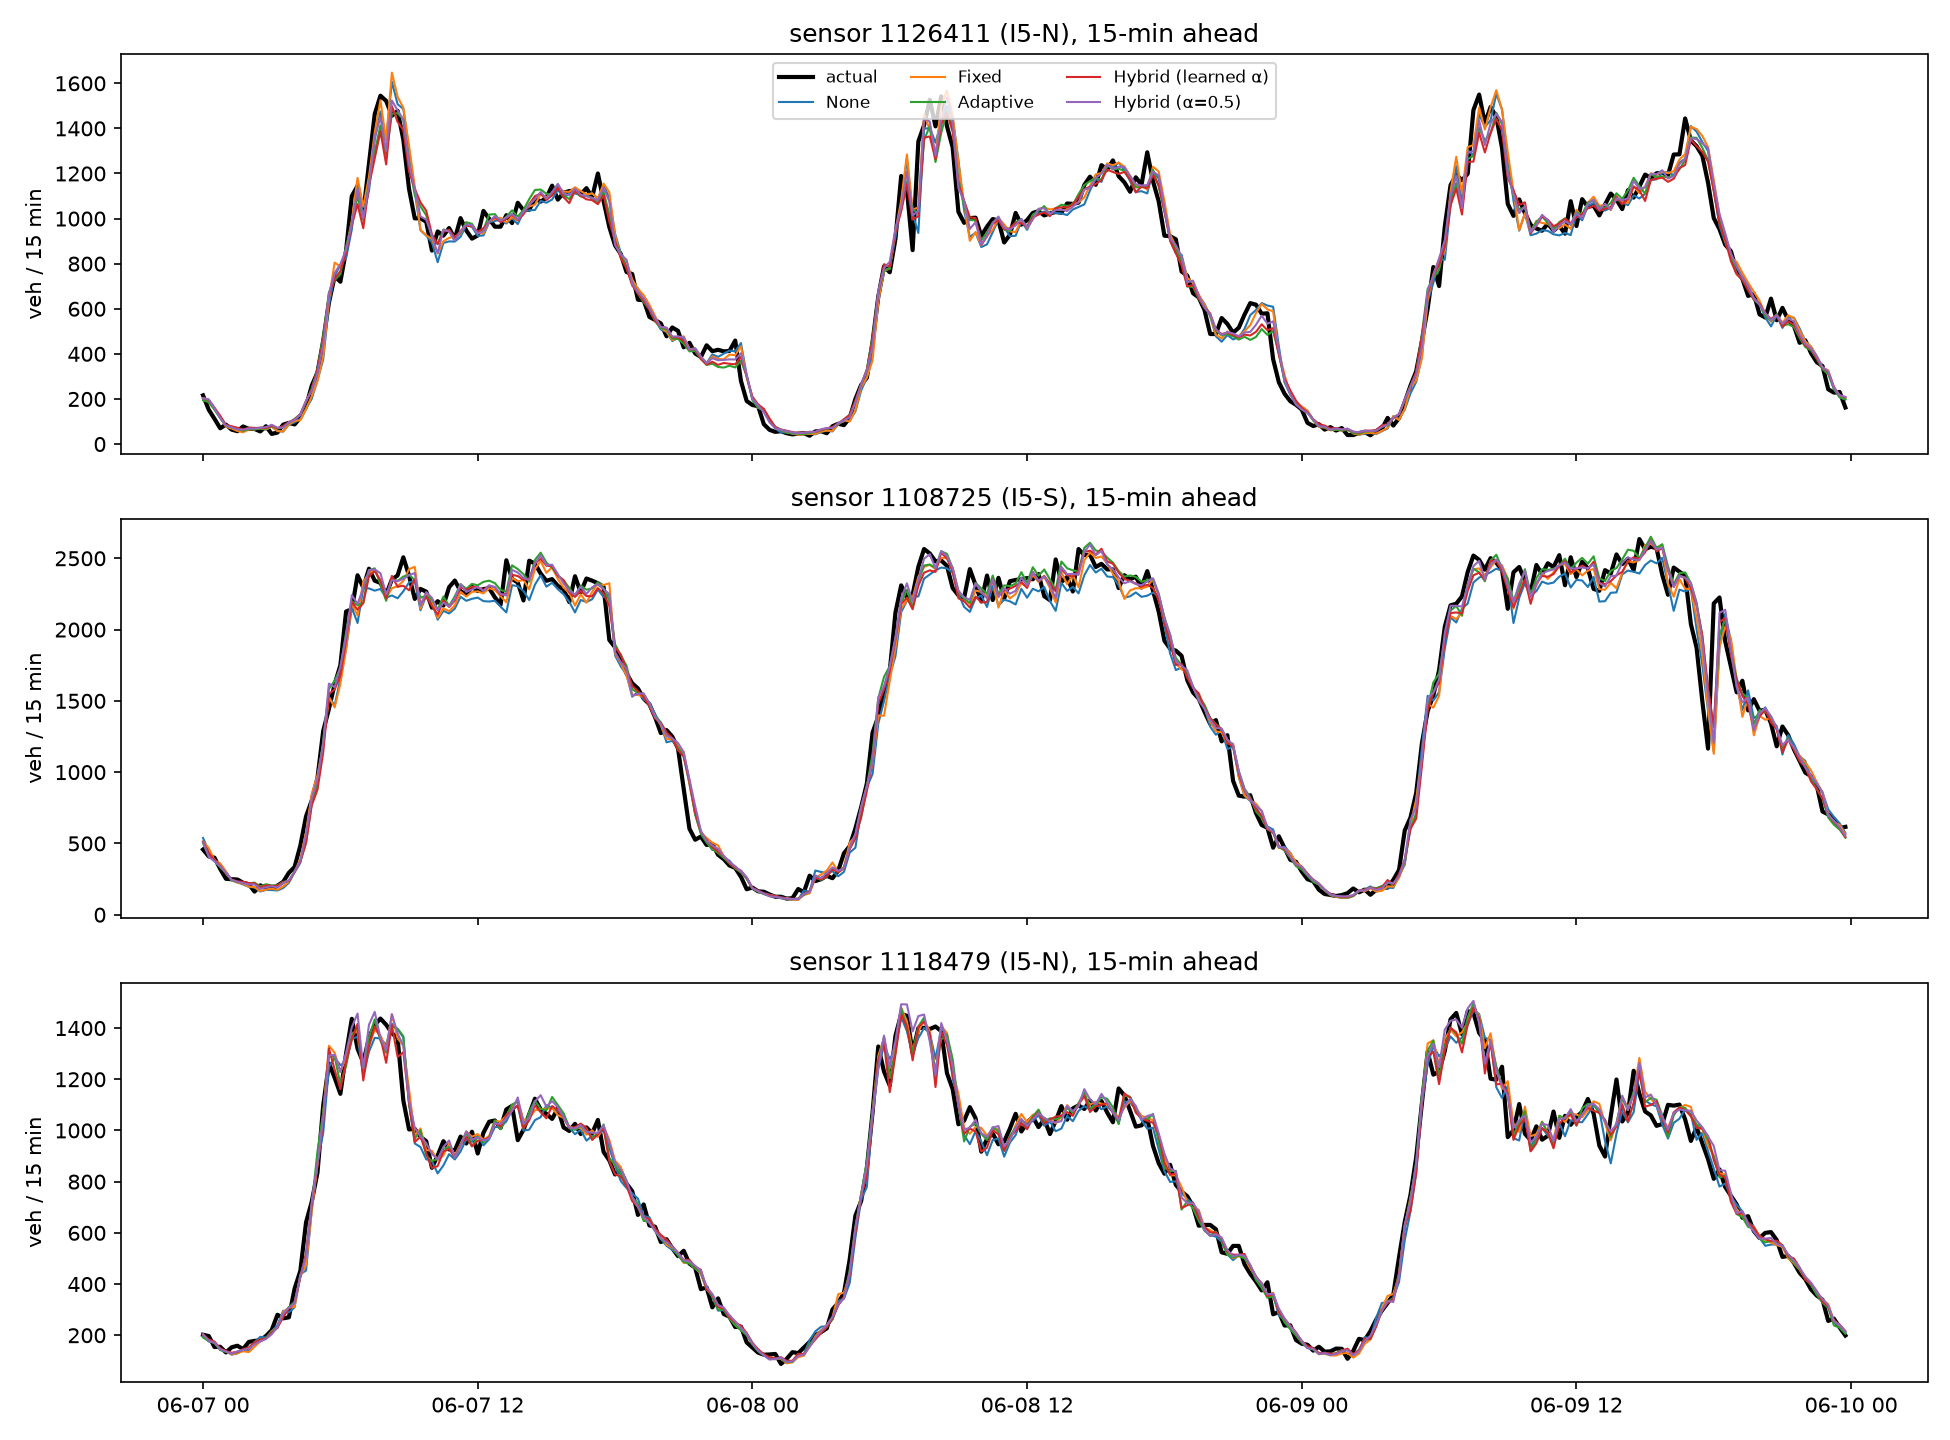
\includegraphics[width=\textwidth]{../figures/q6a_pred_vs_actual_h15.png}
\caption{Predicted vs.\ actual flow, 15 minutes ahead, for three test sensors (7--9 June 2021, Monday--Wednesday).}
\label{fig:pred15}
\end{figure}

\begin{figure}[H]
\centering
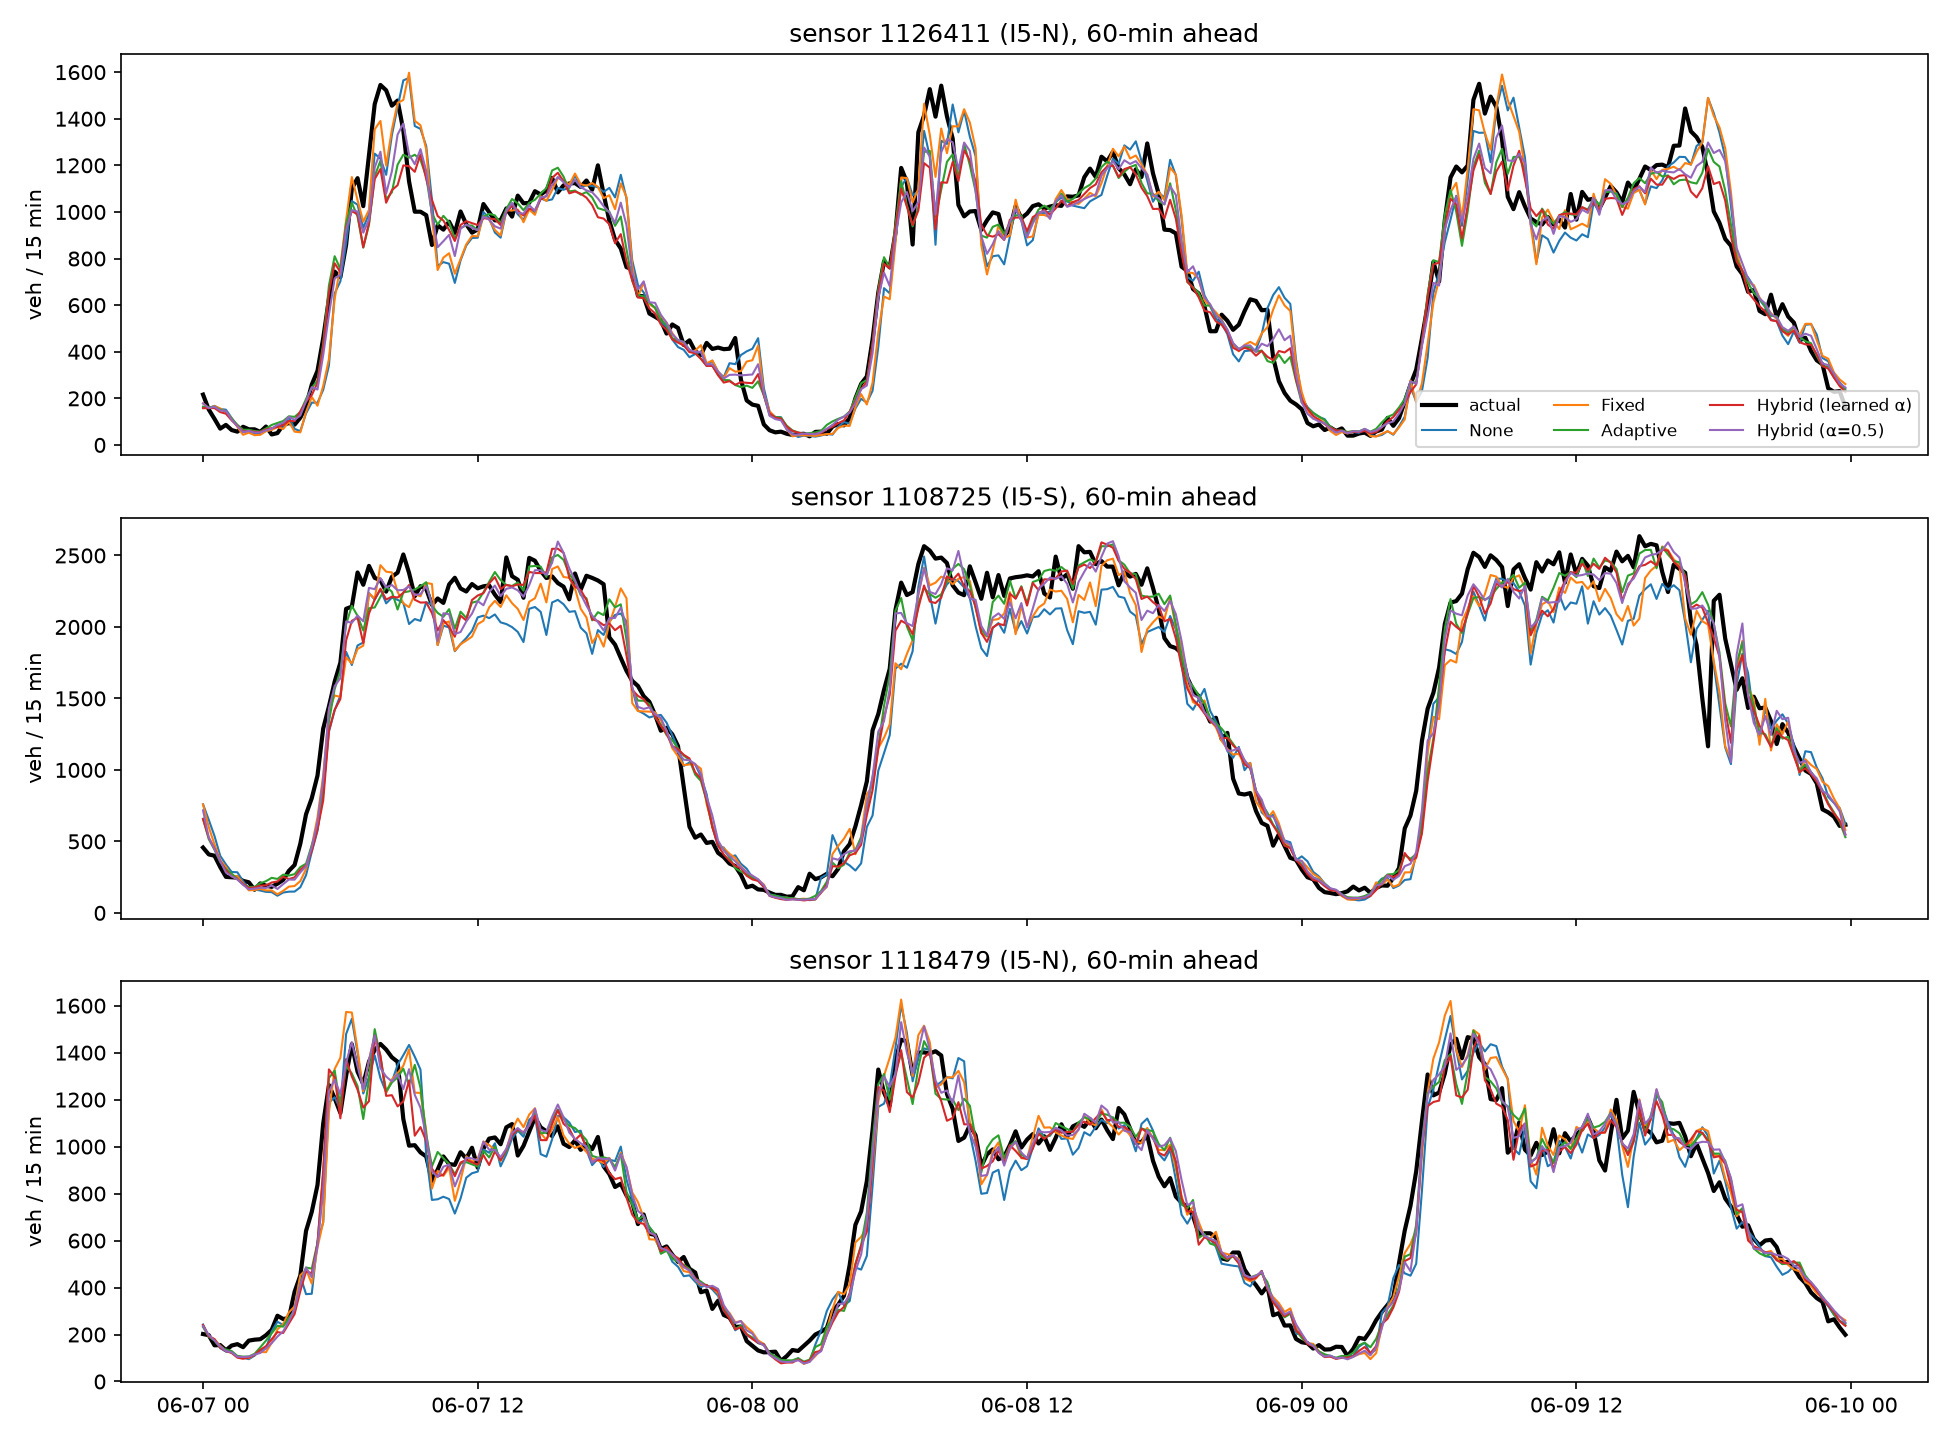
\includegraphics[width=\textwidth]{../figures/q6a_pred_vs_actual_h60.png}
\caption{Predicted vs.\ actual flow, 60 minutes ahead, for the same sensors and days.}
\label{fig:pred60}
\end{figure}

\textbf{Predicted vs.\ actual.} Figures~\ref{fig:pred15} and~\ref{fig:pred60} show three sensors over three weekdays in the test period: the sensor from Q3(c) (1126411, I5 northbound), the busiest fully observed test sensor (1108725, I5 southbound) and a sensor of typical volume (1118479, I5 northbound).
\begin{itemize}
\item \emph{15 minutes ahead}, all models follow the actual flow closely, including the morning peaks and the evening decline, and the lines are hard to tell apart. This matches the small differences at this horizon in Table~\ref{tab:horizon}.
\item \emph{60 minutes ahead}, the differences become visible. The temporal-only (blue) and fixed-graph (orange) predictions tend to lag behind sudden changes: for example, at sensor 1126411 their morning peak on 7 June arrives too late and overshoots. At sensor 1108725 the temporal-only model clearly underestimates the long midday plateau (about 2{,}000--2{,}100 instead of 2{,}300--2{,}500), while the adaptive and hybrid models stay closer to it.
\item No model can predict truly unexpected events. On 9 June around 17:00, sensor 1108725 suddenly drops to about 1{,}150 vehicles. All models miss this and show a similar dip only about an hour later, once it appears in their input window. A drop like this (probably an incident) is not visible in the data in advance.
\end{itemize}

\subsection*{Q6(b) -- Graph structure analysis}

To compare the learned graph (from the adaptive model) with the road graph, I measured four things:
\begin{itemize}
\item \emph{overlap}: how many of each sensor's strongest learned neighbours are also road-graph neighbours;
\item \emph{distance}: the straight-line (great-circle) distance between connected sensors, from their latitude and longitude;
\item \emph{similarity}: the correlation between the two sensors' flows in the training year, after removing each sensor's average weekly pattern (``residual correlation'', as in Q3(c));
\item \emph{concentration}: how much of the total weight goes to the most-used sensors.
\end{itemize}
For each sensor I took its 10 largest learned weights (excluding itself) as its ``learned top-10 neighbours''. For comparison I also used random sensor pairs, since 3.4\% of all pairs are road-graph edges (the density from Q3(b)).

\begin{table}[H]
\centering
\small
\begin{tabular}{@{}lrrr@{}}
\toprule
& Road-graph edges & Learned top-10 & Random pairs \\
\midrule
Share that are road-graph edges        & 100\%  & 3.8\%  & 3.4\% \\
Median distance (km)                   & 2.4    & 22.2   & 23.0 \\
Median residual correlation            & 0.763  & 0.746  & 0.720 \\
Same freeway and direction             & 22.3\% & 10.4\% & 7.1\% \\
\bottomrule
\end{tabular}
\caption{Learned connections compared with road-graph connections and random pairs.}
\label{tab:learned}
\end{table}

\begin{figure}[H]
\centering
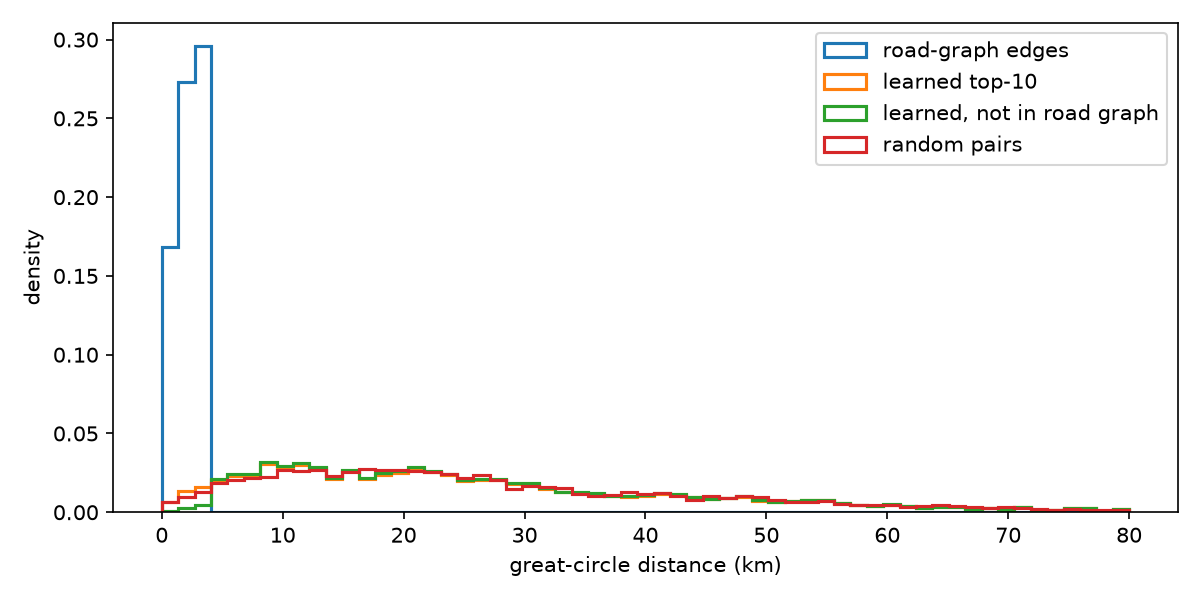
\includegraphics[width=0.85\textwidth]{../figures/q6b_edge_distances.png}
\caption{Distance between connected sensors: road-graph edges, learned top-10 edges, learned edges that are not in the road graph, and random pairs.}
\label{fig:dist}
\end{figure}

\begin{figure}[H]
\centering
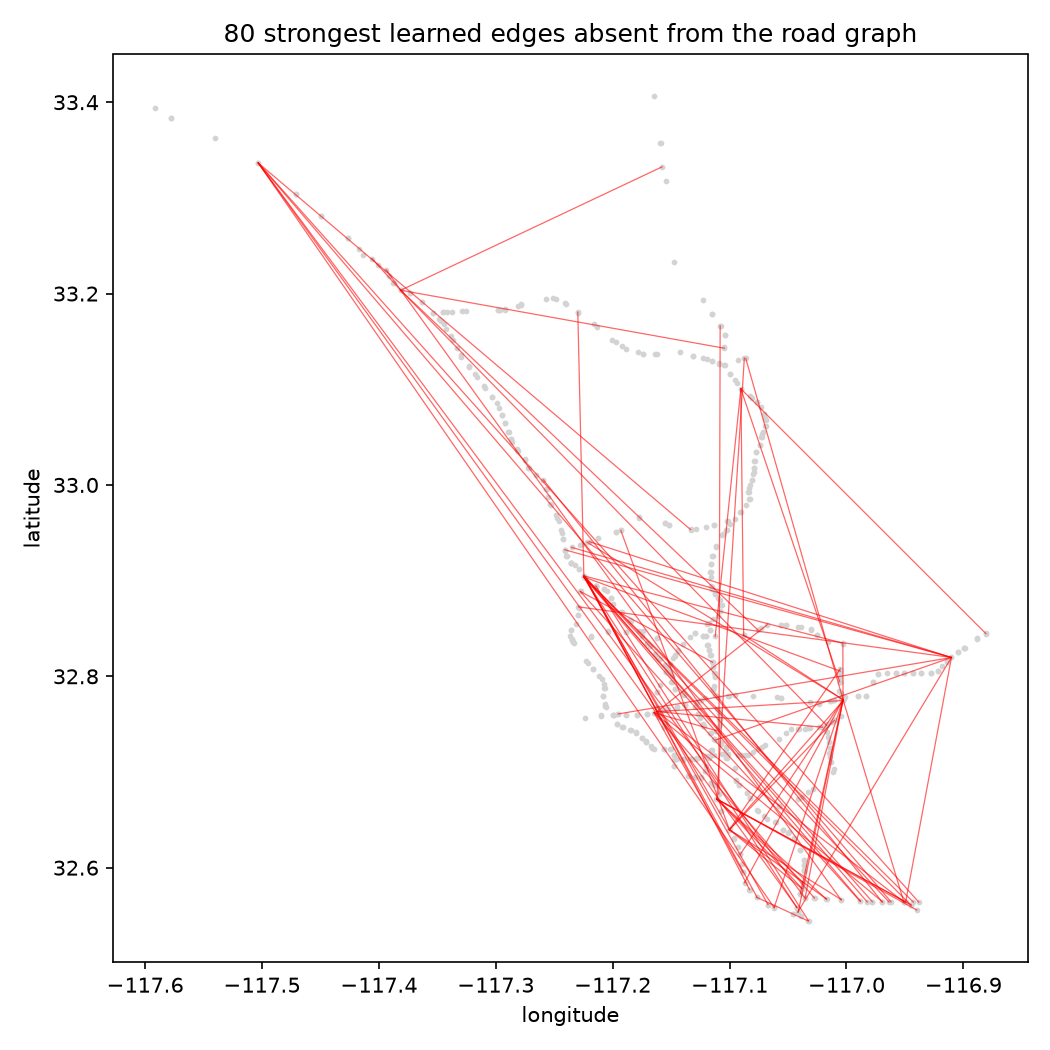
\includegraphics[width=0.6\textwidth]{../figures/q6b_learned_nonphysical_edges.png}
\caption{The 80 strongest learned connections that do not exist in the road graph.}
\label{fig:nonphys}
\end{figure}

\textbf{1. Are the strongest learned connections also in the road graph?} Almost never. Only 4.2\% of each sensor's single strongest learned neighbour, 3.8\% of its top 10, and 4 of the 100 strongest learned connections overall are road-graph edges. Random pairs would give 3.4\%, so the overlap is barely better than chance.

\textbf{2. Are learned connections between nearby sensors?} No. Road-graph edges connect sensors a median of 2.4 km apart, and all of them are within about 4 km (Figure~\ref{fig:dist}). Learned connections are a median of 22.2 km apart, practically the same as random pairs (23.0 km), and their distance distribution in Figure~\ref{fig:dist} lies almost exactly on top of the random one. Figure~\ref{fig:nonphys} shows the same on the map: the strongest learned connections cross the whole county, and many of them meet at a few points.

\textbf{3. Can the learned graph capture dependencies that the road graph misses?} 96\% of the learned connections are not in the road graph, so the model clearly uses relationships the road graph does not contain. But these are only slightly more similar than random pairs (residual correlation 0.745 vs.\ 0.720), and less similar than road neighbours (0.763). So the learned graph is \emph{not} mainly finding hidden pairs of sensors that behave alike. Two further measurements show what it does instead:
\begin{itemize}
\item \textbf{It uses a few hubs.} The 10 most-used sensors receive 11.4\% of all the weight, about 8 times their fair share (1.4\%), and the 50 most-used receive 36.6\% (5 times their share of 7\%). These hubs are the vertical stripes in Figure~\ref{fig:learnedadj} and the star-shaped clusters of lines in Figure~\ref{fig:nonphys}.
\item \textbf{Many hubs are dead sensors.} 12 of the 20 biggest hubs are sensors that never recorded any data. Dead sensors are only 2.7\% of all sensors but receive 16\% of all the weight. Their input is always zero, so their features are the same constant vector at every time step. Sending weight to them is a way for the model to say ``use less information from other sensors here'': each row must sum to 1, and the learned self-weight is about 0 (the residual already carries each sensor's own features), so a dead sensor works as a ``parking spot'' for unused weight. This is similar to the ``attention sinks'' seen in transformers.
\end{itemize}

\textbf{4. Why might a learned graph perform better or worse than the fixed graph?}

It \emph{performed better} here for several reasons:
\begin{itemize}
\item Each sensor averages over about 29 sensors spread across the region (compared with about 14 effective neighbours in the road graph), many of them shared hubs. This gives every sensor a summary of the overall traffic state in San Diego: whether it is a busy or quiet day, how strong the rush hour is, whether there is a holiday. A local 2-km road neighbourhood cannot provide that, and it matters most for longer forecasts, which matches the growing gain with horizon in Table~\ref{tab:horizon}.
\item Each sensor gets its own mix of weights, so the graph can adapt to each sensor individually. With the dead-sensor ``sink'', each sensor can also control how much neighbour information it takes in. The row-normalised road graph cannot do this.
\item The road graph has its own problems for this task: it connects sensors to the opposite carriageway and to dead sensors with fixed weights.
\item The adaptive model has about twice as many parameters, which gives it extra capacity.
\end{itemize}

A learned graph can also \emph{perform worse}:
\begin{itemize}
\item It has to be learned from data, so with little training data it can overfit or learn spurious connections.
\item It depends on the random initialisation, and it cannot adapt when the network changes, for example when a new sensor is added that has no embedding.
\item It is hard to interpret: as this analysis shows, it may rely on artefacts such as dead sensors instead of real traffic relationships.
\item The road graph contains real physical knowledge for free. When data are limited, or for very local effects such as a queue spreading from one sensor to the next, this prior can be more reliable than a learned graph.
\end{itemize}

\subsection*{Q6(c) -- Critical discussion}

\textbf{Does a lower forecasting error mean the learned graph represents actual road connectivity?} No, and these results show it directly. The learned graph gives the lowest error of all models, yet its connections overlap with the road network no more than random pairs would, they are as far apart as random pairs, and many of the most heavily used ``connections'' point to sensors that never recorded any data. The learned matrix is simply whatever weighting helps to reduce the forecasting loss. It works more like a learned way of collecting information from the whole network than like a map of which roads are connected. It is also not unique: many different embeddings $E_1, E_2$ could give similar predictions with very different-looking graphs. A good forecast proves that the graph is \emph{useful}, not that it is \emph{true}.

\textbf{Why might a hybrid graph outperform fixed or adaptive alone?} In principle, the two parts complement each other. The road graph provides reliable, physically meaningful local links (for example, the sensor directly downstream), which the model does not have to learn and which stay valid when data are scarce. The adaptive part adds what the road graph cannot provide, such as region-wide context and links between distant sensors with similar demand. A hybrid can therefore be more accurate than the fixed graph and more stable and interpretable than the purely adaptive one. In my experiments this did \emph{not} happen: the learned $\alpha$ fell to 0.015, and forcing $\alpha = 0.5$ made the results worse. A likely reason is that the road graph, as provided, mixes in opposite carriageways and dead sensors with fixed weights, and that the 30-epoch budget gave enough data to learn a better graph without the prior. A hybrid would be more likely to help with less training data, or with a cleaner road graph (for example, one without dead sensors and without links to the opposite direction).

\textbf{Limitations of a static graph.} Both the road graph and the learned graph are fixed after training: the same weights are used at 3 a.m.\ and at 5 p.m., on weekdays and at weekends. But the relationships between sensors change throughout the day. During rush hour, queues spread from one sensor to the next and neighbours matter a lot; at night traffic flows freely and sensors are almost independent. Incidents, roadworks and events create temporary links that no static graph can represent. The learned graph here also had to average over very different periods, such as the 2020 lockdown and the recovery in 2021. Possible improvements are:
\begin{itemize}
\item a \emph{dynamic} adjacency computed from the current input window (for example with attention), so the graph changes with the traffic state;
\item separate graphs, or graph weights that depend on time of day and day of week;
\item removing dead sensors from the learned graph, or giving the model an explicit self-weight, so it does not need ``sink'' sensors.
\end{itemize}

% ---------------------------------------------------------
% QUESTION 7
% ---------------------------------------------------------
\section*{Question 7 -- Reproducibility and Reporting}

\textbf{Code.} All code is in the GitHub repository linked on the first page. The \texttt{README.md} explains how to set up the environment, how to download the data with the Kaggle command-line tool, and the order in which to run the scripts:
\begin{enumerate}
\item \texttt{data\_prep.py}: SD extraction, resampling, missing values and the adjacency (Q3(a)).
\item \texttt{q3\_graph.py}: graph statistics and neighbourhood analysis (Q3(b), Q3(c)).
\item \texttt{train.py}: training and evaluation (Q4, Q5). The option \texttt{-{}-adj} selects the graph (\texttt{none}, \texttt{fixed}, \texttt{adaptive} or \texttt{hybrid}), and \texttt{-{}-alpha 0.5} gives the fixed-$\alpha$ hybrid. The script \texttt{kaggle\_\allowbreak kernel/\allowbreak run\_\allowbreak all.py} runs all four models on a Kaggle GPU.
\item \texttt{analysis.py}: tables, prediction plots and learned-graph analysis (Q6).
\item \texttt{q1\_verify.py}, \texttt{q2\_ring.py}: checks and figures for Q1 and Q2.
\end{enumerate}
Every training run saves a JSON file in \texttt{results/} with its settings, per-epoch log, validation and test metrics (overall and per horizon), training time and hardware.

\begin{table}[H]
\centering
\small
\begin{tabular}{@{}ll@{}}
\toprule
Setting & Value \\
\midrule
Input / output & 8 steps (2 h) $\to$ 4 steps (1 h), 15-minute resolution \\
Temporal encoder & 2 $\times$ Conv1d (kernel 3, 32 ch., ReLU) + Linear$(256 \to 32)$ \\
Graph layer & $H = \mathrm{ReLU}(\hat{A} Z W_g) + Z$, $W_g \in \mathbb{R}^{32 \times 32}$, one layer \\
Forecast head & Linear$(32 \to 32)$, ReLU, Linear$(32 \to 4)$ \\
Hidden size $d$ / embedding size $d_e$ & 32 / 10 \\
Fixed $\hat{A}$ & $D^{-1}A$ (row normalisation, self-loops already in $A$) \\
Adaptive $\hat{A}$ & $\mathrm{Softmax}_{\text{row}}(\mathrm{ReLU}(E_1 E_2^\top))$, dense \\
Hybrid & $\alpha \hat{A}_{\text{fixed}} + (1-\alpha)\hat{A}_{\text{adaptive}}$; $\alpha$ learned or $0.5$ \\
Loss & masked MAE on z-scored values \\
Optimiser & Adam, learning rate $10^{-3}$, gradient clipping 5.0 \\
Batch size & 64 (549 batches per epoch) \\
Epochs & 30; early stopping (patience 5); best val.\ checkpoint \\
Random seed & 42 (Python, NumPy, PyTorch; deterministic cuDNN) \\
Normalisation & global z-score from observed training values \\
\bottomrule
\end{tabular}
\caption{Hyperparameters, shared by all models.}
\end{table}

\textbf{Hardware and training times.}
\begin{itemize}
\item \textbf{Training:} all models were trained in a Kaggle notebook on one NVIDIA Tesla T4 GPU (16\,GB, CUDA 13.0). All models used the same machine, so their training times are comparable. Each epoch took about 20 seconds (temporal-only) to 22 seconds (adaptive and hybrid).
\item \textbf{Preprocessing and analysis:} a local Linux machine (CPU only).
\end{itemize}
Measured training times (30 epochs, including validation after every epoch) are in Table~\ref{tab:final}: 10.0 minutes (temporal-only), 10.4 minutes (fixed), 10.9 minutes (adaptive), 10.9 minutes (hybrid with learned $\alpha$) and 10.7 minutes (hybrid with $\alpha = 0.5$).

% ---------------------------------------------------------
% GENERATIVE AI USAGE (MANDATORY SECTION)
% ---------------------------------------------------------
\section*{Generative AI Usage}

\textit{Generative AI tools were utilized during the completion of this assignment strictly as supplementary assistants. Primarily, AI was used as a learning aid to deepen my understanding of the assignment's underlying concepts, as well as to break down the specific architectures and techniques required for the tasks.} 

\textit{Furthermore, these tools provided support in the drafting and grammatical refinement of this report, debugging and structuring programming code, and compiling supporting evidence. However, all core ideas, critical analyses, experimental methodologies, and final implementations presented in this document are entirely my own original work. The AI was leveraged to facilitate execution and conceptual clarity, not to replace independent critical thinking or problem-solving.}

\end{document}
